\documentclass{scrreprt}
\usepackage[utf8]{inputenc}
\usepackage{booktabs}
\usepackage{xcolor}
\usepackage{hyperref}
\usepackage{lmodern}
\usepackage[T1]{fontenc}
\usepackage{textcomp}
\usepackage{geometry}
\usepackage{float}
\usepackage{array}
\geometry{a4paper, margin=1in}
\usepackage{placeins} 
\usepackage{graphicx}
\usepackage{tabularx} %
\usepackage{longtable} %
\usepackage{array} %
\usepackage{ragged2e}
\usepackage{float} % 
\usepackage{multirow}
\usepackage{pgffor}

\newcounter{sprint}
\setcounter{sprint}{0}
\usepackage{longtable}
\usepackage{array}
\usepackage{multirow}

\hypersetup{
    pdftitle={Software Planning and UML},
    pdfauthor={Team 3 - PAO 2 2024},
    pdfsubject={TeX and LaTeX},
    pdfkeywords={TeX, LaTeX, graphics, images},
    colorlinks=true,
    linkcolor=blue,
    citecolor=black,
    filecolor=black,
    urlcolor=purple,
    linktoc=page
}
\def\myversion{1.0 }
\date{November 14, 2024}

\begin{document}

\begin{titlepage}
    \begin{flushright}
        \rule{16cm}{1.5pt} \\[1cm]
        {\Huge\bfseries SOFTWARE PLANNING\\ AND UML (Approved)}\\[1cm]
        {\LARGE\bfseries for}\\[1cm]
        {\Huge\textbf{ESPOLTEL HIRING MANAGER}}\\[2cm]
        {\Large\textbf{Version \myversion}}\\[1.5cm]
        
        {\Large\textbf{Jeremy Rodrigo Poveda Gorotiza}\\
        \textbf{José David Ramos Rios}\\
        \textbf{Diego Fernando Flores Rengifo}\\
        \textbf{Ariana Valentina Palacios Saenz}\\
        \textbf{Alex Javier Vizuete Pereira}}\\[1.5cm]
        
        {\Large\textbf{Submitted to:} Francisco Ramirez}\\[1.5cm]
        {\Large\textbf{\today}}
    \end{flushright}
    \vfill
\end{titlepage}

\chapter*{Revision History}
\setcounter{page}{1}
\begin{center}
	\begin{tabular}{@{} l l p{6.5cm} l @{}}
		\toprule
		\textbf{Name}    & \textbf{Date}   & \textbf{Reason for Changes} & \textbf{Version} \\ 
		\midrule
		Team 3           & 2025-1-10      & Initial draft               & 1.0              \\
		\bottomrule
	\end{tabular}
\end{center}

\tableofcontents

\listoffigures
\listoftables



\chapter{Introduction}
\section{Summary}
This document presents a comprehensive framework for the design, planning, and execution of the ESPOLTEL HIRING MANAGER system. This product integrates a robust risk management strategy, a detailed project execution timeline, and a structured Sprint Backlog plan. Through the inclusion of Unified Modeling Language (UML) diagrams, we provide a thorough representation of both the static and behavioral logic of the system, ensuring that the architecture adheres to SOLID principles and eliminates implementation inefficiencies.

Our primary objective is to meticulously define the planning and breakdown of the system’s static structure, logical flow, behavioral processes, implementation strategies, and activity sequences. These components collectively support the realization of a user-centric, scalable, and maintainable product.

\section{Key features and Objetives}
The ESPOLTEL HIRING MANAGER product is designed to streamline and enhance the recruitment process, leveraging a combination of web and mobile modules for maximum efficiency. Key objectives include:

\begin{enumerate}
	\item \textbf{Risk Mitigation:} Developing a proactive risk management plan to address potential challenges in implementation and deployment.
	\item \textbf{Comprehensive Planning:} Structuring the project execution into manageable phases using Agile methodologies.
	\item \textbf{System Design:} Crafting static and behavioral UML diagrams to visualize the architecture, interactions, and workflows.
	\item \textbf{Adherence to SOLID Principles:} Ensuring maintainability and scalability by avoiding anti-patterns and promoting clean code practices.
\end{enumerate}

\chapter{Risk management, product and sprint backlogs and scheduling}
\section{Risk management}
In this section, we will identify, quantify, and classify the various risks that may arise during the software development process. Additionally, we will provide a detailed assessment of the likelihood of occurrence, the potential impact of each risk, and the corresponding protocols to be followed in the event they materialize.

%%
\begin{table}[h!]
	\centering \small
	\renewcommand{\arraystretch}{1.5} 
	\begin{tabular}{|p{10cm}|p{5cm}|} 
		\hline
		\textbf{Description} & \textbf{Probability Range} \\ \hline
		Not Probable: The event is highly unlikely to occur. & 0\% - 20\% \\ \hline
		Low Probability: The event is unlikely but possible. & 21\% - 40\% \\ \hline
		Moderate Probability: The event has an even chance of occurring. & 41\% - 60\% \\ \hline
		High Probability: The event is likely to occur. & 61\% - 80\% \\ \hline
		Very High Probability: The event is almost certain to occur. & 81\% - 100\% \\ \hline
	\end{tabular}
	\caption{Probability of Occurrence}
\end{table} \FloatBarrier
%%

%%

%%
\begin{table}[h!]
	\centering \small
	\renewcommand{\arraystretch}{1.5} 
	\begin{tabular}{|p{5cm}|p{10cm}|} 
		\hline
		\textbf{Impact Level} & \textbf{Description} \\ \hline
		Low Impact & Minimal effect on the project. No significant changes required. \\ \hline
		Moderate Impact & Some delays or adjustments needed but manageable within the team. \\ \hline
		High Impact & Significant disruptions, requiring immediate attention and resource allocation. \\ \hline
		Critical Impact & Severe consequences on project delivery, with major delays or failure possible. \\ \hline
	\end{tabular}
	\caption{Impact Levels}
\end{table} \FloatBarrier
%%
The following table outlines the identified risks associated with the project, including their probability of occurrence, potential impact, and the corresponding action protocol.
%%
\begin{table}[h!]
	\centering \small
	\renewcommand{\arraystretch}{1.5}
	\begin{tabular}{|p{.75cm}|p{4cm}|p{2.5cm}|p{2.5cm}|p{4.75cm}|} 
		\hline
		\textbf{Id} & \textbf{Name} & \textbf{Probability} & \textbf{Impact} & \textbf{Action Protocol} \\ \hline
		001 & Changes in requirements after development completion & High Probability & High Impact & Establish a communication protocol to clarify that no new requirements will be accepted after the design phase is finalized. \\ \hline
		002 & Discovery of implicit requirements not considered in the design & Very High Probability & High Impact & Accept and address the risk by updating the design and implementing the missing requirements. \\ \hline
		003 & Need for developer training & High Probability & High Impact & Provide immediate training on the required frameworks to minimize delays and ensure smooth development progress. \\ \hline
		004 & Difficulty understanding prior implementation, causing delays & Low Probability & Critical Impact & Reduce the probability by consulting previous implementers to gain insights into the system before development begins. \\ \hline
		005 & Schedule misalignment affecting task timelines & Not Probable & High Impact & Mitigate the risk by redistributing tasks and holding regular progress meetings to stay on track. \\ \hline
		006 & Performance drop due to prior monolithic architecture & Low Probability & High Impact & Accept the risk, inform the client, and propose alternative solutions to improve performance. \\ \hline
		007 & Database schema not designed for extensions & Low Probability & Moderate Impact & Accept the risk and adapt the existing schema to accommodate the new requirements. \\ \hline
		008 & Insufficient documentation provided by the client & High Probability & Critical Impact & Reduce probability by maintaining active communication with the client to obtain necessary documentation. \\ \hline
	\end{tabular}
	\caption{Risk Assessment and Action Protocols}
\end{table} \FloatBarrier
%%

\section{Product backlog}
\begin{longtable}{|p{0.8cm}|p{1.5cm}|p{2.5cm}|p{8cm}|p{2cm}|} \hline
	\textbf{ID} & \textbf{Priority} & \textbf{Dependencies} & \textbf{Item} & \textbf{Estimation (hours)} \\ \hline
	\endfirsthead
	\hline
	\textbf{ID} & \textbf{Priority} & \textbf{Dependencies} & \textbf{Item} & \textbf{Estimation (hours)} \\ \hline
	\endhead
	PB1 & 0 & None & Research Spring Boot  platform: Investigation of the architecture, modules, and functionalities of Spring Boot relevant to the project. Includes feasibility evaluation and the creation of a document with findings and recommendations. & 4 \\ \hline
	PB2 & 0 & None & Definition of the database schema: Design the database schema, including the definition of tables, relationships, and constraints. An Entity-Relationship diagram and the SQL script for database creation will be generated. & 8 \\ \hline
	
	%Register and loggin into the system
	
	PB3 & 1 & PB1, PB2 & \textbf{As} a user of ESPOLTEL Hiring Manager, \textbf{I want} to create my own account \textbf{so that} I can access all controls related to my role, ensuring my information and permissions are separate from other users. & 6 \\ \hline
	PB4 & 1 & PB3 & \textbf{As} a user of ESPOLTEL Hiring Manager, \textbf{I want} to verify my email address upon registration \textbf{so that} I can ensure secure access to the system and confirm my identity. & 8 \\ \hline
	PB5 & 2 & PB3 & \textbf{As} a user of ESPOLTEL Hiring Manager, \textbf{I want} to create my own account using the mobile app, \textbf{so that} I can access all controls corresponding to my role, and ensure that my information and permissions are separate from those of other users. & 6 \\ \hline
	PB6 & 1 & PB5 & \textbf{As} a user of ESPOLTEL Hiring Manager, \textbf{I want} to verify my email address when registering from my mobile device, \textbf{so that} I can ensure secure access to the system and confirm my identity. & 10 \\ \hline
	PB7 & 1 & PB3 & \textbf{As} a user of ESPOLTEL Hiring Manager, \textbf{I want} to log in securely using my credentials \textbf{so that} I can access features and project management tools. & 4\\ \hline
	PB8 & 1 & PB7 & \textbf{As} a user of ESPOLTEL Hiring Manager, \textbf{I want} to select my role (Aspirant, Project Manager, Project Director, or HR member) before logging in \textbf{so that} I am directed to the appropriate login process and access functionalities specific to my role. & 6 \\ \hline
	PB9 & 2 & PB7 & \textbf{As} a user of ESPOLTEL, \textbf{I want} to securely log in to the system using my credentials on my mobile device, \textbf{so that} I can access the appropriate functions and features according to my user role. & 5 \\ \hline
	PB10 & 2 & PB8 & \textbf{As} a user of ESPOLTEL, \textbf{I want} to be able to select my role (Aspirant, Project Manager, Project Director, or HR member) on my mobile device before logging in, \textbf{so that} I can be directed to the specific features and functionalities relevant to my role. &  6 \\ \hline
	PB11 & 3 & PB3 & \textbf{As} a user of ESPOLTEL Hiring Manager, \textbf{I want} to be able to recover my password through a secure and efficient process if I forget it, \textbf{so that} I can regain access to the system and continue with my responsibilities without delay. & 5 \\ \hline
	PB12 & 3 & PB5 & \textbf{As} a user of ESPOLTEL Hiring Manager, \textbf{I want} to be able to recover my password through a secure and efficient process by email from my mobile device if I forget it, \textbf{so that} I can regain access to the system and continue with my responsibilities without delay. & 6 \\ \hline
	
	%% Signer and FirmaEC
	PB13 & 2 & PB1,PB2 & \textbf{As} an aspirant or manager, \textbf{I want} to have access to contracts or confidential agreements pending my signature, \textbf{so that} I can review and sign them digitally within the web application. & 12 \\ \hline
	PB14 & 1 & P13 & \textbf{As} an aspirant, \textbf{I want} to upload my digital certificate to the platform \textbf{so that} I can sign documents such as contracts or confidentiality agreements for the projects I have applied to. & 5 \\ \hline
	PB15 & 1 & P13 & \textbf{As} a manager, \textbf{I want} to upload my digital certificate to the platform \textbf{so that} I can sign multiple documents such as contracts or confidentiality agreements for the projects I manage. & 5 \\ \hline
	PB16 & 1 & P14 & \textbf{As} an aspirant, \textbf{I want} to digitally sign my contract and confidentiality agreement \textbf{so that} I can complete the paperwork required for my hiring process. & 12 \\ \hline
	PB17 & 1 & P15 & \textbf{As} a manager, \textbf{I want} to digitally sign multiple documents, such as contracts or confidentiality agreements, simultaneously, \textbf{so that} I can save time and work more efficiently. & 12 \\ \hline
	PB18 & 3 & PB16 & \textbf{As} an aspirant, \textbf{I want} to view the contracts of the projects I have applied for and that are currently active, \textbf{so that} I have a clear view of the agreements I have signed. & 6 \\ \hline
	PB19 & 3 & PB18 & \textbf{As} an aspirant, \textbf{I want} to download the contracts of the projects I have applied for and that are currently active, \textbf{so that} I have a record of the agreements I have signed. & 4 \\ \hline
	PB20 & 3 & PB16 & \textbf{As} an aspirant, \textbf{I want} to view the contracts of the projects I have applied for and that are currently active on my smartphone, \textbf{so that} I have a clear view of the agreements I have signed. & 6 \\ \hline
	PB21 & 3 & PB20 & \textbf{As} an aspirant, \textbf{I want} to download the contracts of the projects I have applied for and that are currently active on my smartphone, \textbf{so that} I have a record of the agreements I have signed. & 4 \\ \hline
	PB22 & 1 & PB16 & \textbf{As} an HR member, \textbf{I want} to validate the digital signatures of aspirants \textbf{so that} I can ensure contracts and agreements are formalized. & 8 \\ \hline
	
	%% Project creation 
	PB23 & 2 & PB3 & \textbf{As} a project manager, \textbf{I want} to create a project by defining its name, description, start date, end date, and type, \textbf{so that} the project's objectives and timeline are clearly established. & 12 \\ \hline
	PB24 & 2 & PB23 & \textbf{As} a project manager, \textbf{I want} to define roles and profiles required for the project, including necessary skills and experience for each profile, \textbf{so that} aspirants can understand the requirements and apply to suitable positions. & 6 \\ \hline
	PB25 & 3 & PB24 & \textbf{As} a Director, \textbf{I want} to recommend an aspirant who has previously worked for ESPOLTEL for a role in a project, based on their past performance and experience, \textbf{so that} I have a worker I trust in my project. & 8 \\ \hline
	PB26 & 2 & PB24 & \textbf{As} an HR member, \textbf{I want} to validate the profiles created by project directors \textbf{so that} I can edit, approve, the profiles and positions defined for a project, ensuring they align with the company's standards and requirements. & 12 \\ \hline
	PB27 & 2 & PB23 & \textbf{As} a project manager or director at ESPOLTEL, \textbf{I want} to monitor on my smartphone the projects under my supervision, \textbf{so that} I can maintain better control and make informed decisions. & 8 \\ \hline
	PB28 & 2 & PB23 & \textbf{As} a Director or Manager, \textbf{I want} to view the resources and budget assigned to my project, \textbf{so that} I can track project expenses and resource utilization. & 10 \\ \hline
	%%

	%Apply for a project aspirant
	PB29 & 1 & PB8 & \textbf{As} an aspirant, \textbf{I want} to apply for a position in a project of interest where I meet the required profile \textbf{so that} I can obtain the desired position. & 10 \\ \hline
	PB30& 2 & PB29 & \textbf{As} an aspirant, \textbf{I want} to cancel my postulation for a specific role or hiring profile, \textbf{so that} I can withdraw from a recruitment process if my circumstances change. & 8 \\ \hline
	
	%% Interviews
	PB31& 2 & PB8, PB29& \textbf{As} an HR member, \textbf{I want} to schedule interviews with aspirants, specifying the date, time, and interviewer, \textbf{so that} the selection process can be efficiently conducted. & 10 \\ \hline
	PB32 & 2 & PB31 & \textbf{As} a HR member, \textbf{I want} to record interview results and observations, including scores and comments, \textbf{so that} there is a formal record of each aspirant's evaluation. & 8 \\ \hline
	PB33 & 2 & PB24, PB29 & \textbf{As} an HR member, \textbf{I want} to verify the requirements based on the information of an aspirant, \textbf{so that} I can ensure they meet the necessary qualifications for a project. & 8 \\ \hline
	PB34& 3 & PB32 & \textbf{As} an HR member, \textbf{I want} to add private comments in aspirants' postulations \textbf{so that} I can keep a record of observations and notes during the selection process. & 4 \\ \hline
	PB35 & 2 & PB32, PB33, PB34 & \textbf{As} an HR member, \textbf{I want} to select the best aspirants based on interview results and fulfilled requirements, \textbf{so that} I can identify the most suitable candidates for each role. & 10 \\ \hline
	
	%%Generate format documents
	PB36 & 2 & PB8 & \textbf{As} an HR member, \textbf{I want} to create and manage forms for pre-hiring and hiring processes, defining mandatory fields and document uploads, \textbf{so that} aspirants can provide the necessary information. & 15 \\ \hline
	PB37 & 2 & PB8 & \textbf{As} an HR member, \textbf{I want} to upload templates for contracts and agreements, \textbf{so that} appropriate templates are available for generating personalized documents for aspirants. & 12 \\ \hline
	PB38 & 2 & PB29, PB36 & \textbf{As} an aspirant, \textbf{I want} to upload my personal documents (such as CV, ID, certificates, etc.) and relevant information \textbf{by completing forms defined by HR,} \textbf{so that} I can fulfill postulation requirements. & 8 \\ \hline
	PB39 & 2 & PB37 & \textbf{As} an HR member, \textbf{I want} to generate contracts and agreements from templates, \textbf{so that} I can save time in creating personalized documents. & 12 \\ \hline
	
	%%Search and filter
	PB40 & 2 & PB32, PB33, PB34  & \textbf{As} an HR member, \textbf{I want} to view aspirants by specific skills and experience, \textbf{so that} I can make it easier to select candidates who meet the project requirements. & 4 \\ \hline
	PB41 & 2 & PB8 & \textbf{As} a Director, HR Member, or Manager, \textbf{I want} to view the hires or personnel associated with a project, \textbf{so that} I have an overview of the team composition and recruitment progress. & 10 \\ \hline
	PB42 & 2 & None & \textbf{As} a user of ESPOLTEL Hiring Manager, \textbf{I want} to be able to search and filter information across the platform, including projects, aspirants, roles, documents, and other relevant data, \textbf{so that} I can quickly find and focus on the data I need. & 8 \\ \hline
	
	%Notifications 
	PB43 & 1 & PB10 & \textbf{As} a user of the ESPOLTEL Hiring Manager mobile app, \textbf{I need} to receive notifications for any important events in the recruitment process, \textbf{so that} I can stay informed and respond promptly. & 12 \\ \hline
	PB44 & 2 & PB8 & \textbf{As} an aspirant, \textbf{I want} to monitor on my smartphone the projects I have applied for, \textbf{so that} I can stay updated on their progress and better manage my involvement. & 10 \\ \hline
	PB45 & 2 & PB31 & \textbf{As} an aspirant, \textbf{I want} to receive notifications about my scheduled interviews, including reminders and updates, \textbf{so that} I can be prepared and attend interviews on time. & 8 \\ \hline
	
	%% Testing
	PB46 & 4 & PB45 & Testing and deployment& 24\\ \hline
	\caption{Product Backlog of ESPOLTEL Hiring Manager}
\end{longtable}

\section{Sprint backlog}
The project sprints will be 4 organized for 3 weeks duration.

\begin{longtable}{|p{1.5cm}|p{5.5cm}|p{4.5cm}|p{3cm}|} \hline
	\textbf{Product Backlog Item} & \textbf{User Story} & \textbf{Tasks} & \textbf{Assigned To} \\ \hline
	\endfirsthead
	\hline
	\textbf{Product Backlog Item} & \textbf{User Story} & \textbf{Tasks} & \textbf{Assigned To} \\ \hline
	\endhead
	
	PB1 & Research Spring Boot platform (4 hours) & 

	-Research architecture, modules, and functionalities of Spring Boot. - 3 hours\newline
	-Feasibility evaluation of this framework. - 1 hour 
	&
	- Jeremy Poveda, Diego Flores, Ariana Palacios\newline
	- Alex Vizuete, Jose Ramos
	\\ \hline
	
	PB2 & Definition of the database schema (8 hours) & 
	-Design the database schema (tables, relationships, and constraints). - 4 hours\newline
	-Generate Entity-Relationship diagram and SQL script. - 4 hours
	&
	- Diego Flores, Ariana Palacios\newline
	- Jeremy Poveda, Alex Vizuete
	\\ \hline
	PB3 & \textbf{As} a user of ESPOLTEL Hiring Manager, \textbf{I want} to create my own account \textbf{so that} I can access all controls related to my role, ensuring my information and permissions are separate from other users. (6 hours) & 
	- Design UI for user registration (web). - 2 hours \newline
	- Implement backend logic for user registration and role management. - 3 hours \newline
	- Database integration for user accounts. - 1 hour 
	&
	- Jeremy Poveda \newline
	- Jose Ramos \newline
	- Ariana Palacios
	\\ \hline
	
	PB4 & \textbf{As} a user of ESPOLTEL Hiring Manager, \textbf{I want} to verify my email address upon registration \textbf{so that} I can ensure secure access to the system and confirm my identity. (8 hours) & 
	- Implement email sending functionality (e.g., using Spring Mail). - 3 hours \newline
	- Create email verification endpoint. - 3 hours \newline
	- Integrate email verification with registration flow. - 2 hours
	&
	- Alex Vizuete \newline
	- Diego Flores \newline
	- Jeremy Poveda
	\\ \hline
	
	PB5 & \textbf{As} a user of ESPOLTEL Hiring Manager, \textbf{I want} to create my own account using the mobile app, \textbf{so that} I can access all controls corresponding to my role, and ensure that my information and permissions are separate from those of other users. (6 hours) & 
	- Design UI for user registration (mobile). - 2 hours \newline
	- Implement backend logic for user registration and role management (mobile). - 3 hours \newline
	- Database integration for user accounts (mobile). - 1 hour
	&
	- Diego Flores \newline
	- Jose Ramos \newline
	- Ariana Palacios
	\\ \hline
	
	PB6 & \textbf{As} a user of ESPOLTEL Hiring Manager, \textbf{I want} to verify my email address when registering from my mobile device, \textbf{so that} I can ensure secure access to the system and confirm my identity. (10 hours) & 
	- Adapt email sending functionality for mobile. - 3 hours \newline
	- Create email verification endpoint (mobile). - 4 hours \newline
	- Integrate email verification with mobile registration flow. - 3 hours
	&
	- Alex Vizuete \newline
	- Jeremy Poveda \newline
	- Jose Ramos
	\\ \hline
	
	PB7 & \textbf{As} a user of ESPOLTEL Hiring Manager, \textbf{I want} to log in securely using my credentials \textbf{so that} I can access features and project management tools. (4 hours)& 
- Design UI for user login (web). - 1 hour \newline
- Implement backend logic for authentication. - 2 hours \newline
- Implement session management. - 1 hour
&
- Jose Ramos \newline
- Ariana Palacios \newline
- Alex Vizuete
\\ \hline

PB8 & \textbf{As} a user of ESPOLTEL Hiring Manager, \textbf{I want} to select my role (Aspirant, Project Manager, Project Director, or HR member) before logging in \textbf{so that} I am directed to the appropriate login process and access functionalities specific to my role. (6 hours) & 
- Design UI for role selection. - 3 hours \newline
- Implement role-based access control logic. - 3 hours
&
- Diego Flores \newline
- Jeremy Poveda
\\ \hline
PB9 & \textbf{As} a user of ESPOLTEL, \textbf{I want} to securely log in to the system using my credentials on my mobile device, \textbf{so that} I can access the appropriate functions and features according to my user role. (5 hours) &
- Design UI for user login (mobile). - 2 hours \newline
- Implement backend logic for authentication (mobile). - 2 hours \newline
- Implement session management (mobile). - 1 hour
&
- Jeremy Poveda \newline
- Ariana Palacios \newline
- Alex Vizuete
\\ \hline

PB10 & \textbf{As} a user of ESPOLTEL, \textbf{I want} to be able to select my role (Aspirant, Project Manager, Project Director, or HR member) on my mobile device before logging in, \textbf{so that} I can be directed to the specific features and functionalities relevant to my role. (6 hours) & 
- Design UI for role selection (mobile). - 3 hours \newline
- Implement role-based access control logic (mobile). - 3 hours
&
- Diego Flores \newline
- Jose Ramos
\\ \hline

PB11 & \textbf{As} a user of ESPOLTEL Hiring Manager, \textbf{I want} to be able to recover my password through a secure and efficient process if I forget it, \textbf{so that} I can regain access to the system and continue with my responsibilities without delay. (5 hours) & 
- Design UI for password recovery. - 2 hours \newline
- Implement backend logic for password recovery. - 3 hours
&
- Jose Ramos \newline
- Ariana Palacios
\\ \hline
PB12 & \textbf{As} a user of ESPOLTEL Hiring Manager, \textbf{I want} to be able to recover my password through a secure and efficient process by email from my mobile device if I forget it, \textbf{so that} I can regain access to the system and continue with my responsibilities without delay. (6 hours) &
- Design UI for password recovery (mobile). - 2 hours \newline
- Implement backend logic for password recovery, including email sending (mobile). - 3 hours\newline
- Integrate password recovery with mobile login flow. - 1 hour
&
- Diego Flores \newline
- Ariana Palacios \newline
- Alex Vizuete
\\ \hline

\caption{Sprint 1 of ESPOLTEL Hiring Manager}
\end{longtable}

%%Sprint 2
\begin{longtable}{|p{1.5cm}|p{5.5cm}|p{4.5cm}|p{3cm}|} \hline
	\textbf{Product Backlog Item} & \textbf{User Story} & \textbf{Tasks} & \textbf{Assigned To} \\ \hline
	\endfirsthead
	\hline
	\textbf{Product Backlog Item} & \textbf{User Story} & \textbf{Tasks} & \textbf{Assigned To} \\ \hline
	\endhead
	
	PB13 & \textbf{As} an aspirant or manager, \textbf{I want} to have access to contracts or confidential agreements pending my signature, \textbf{so that} I can review and sign them digitally within the web application. (12) &
	
	Design UI for contract/agreement viewing. - 4 hours \newline
	Implement backend logic for fetching pending documents. - 4 hours \newline
	Integrate digital signature service/library. - 4 hours &
	Jeremy Poveda \newline
	Jose Ramos \newline
	Alex Vizuete \\ \hline
	
	PB14 & \textbf{As} an aspirant, \textbf{I want} to upload my digital certificate to the platform \textbf{so that} I can sign documents such as contracts or confidentiality agreements for the projects I have applied to. (5) &
	
	Design UI for digital certificate upload. - 2 hours \newline
	Implement backend logic for certificate storage and validation. - 3 hours &
	Diego Flores \newline
	Ariana Palacios \\ \hline
	
	PB15 & \textbf{As} a manager, \textbf{I want} to upload my digital certificate to the platform \textbf{so that} I can sign multiple documents such as contracts or confidentiality agreements for the projects I manage. (5) &
	
	Design UI for digital certificate upload (Manager). - 2 hours \newline
	Implement backend logic for certificate storage and validation (Manager). - 3 hours &
	Jeremy Poveda \newline
	Alex Vizuete \\ \hline
	
	PB16 & \textbf{As} an aspirant, \textbf{I want} to digitally sign my contract and confidentiality agreement \textbf{so that} I can complete the paperwork required for my hiring process. (12) & 
	
	Integrate digital signature functionality for aspirants. - 6 hours \newline
	Design UI for signing contracts and agreements. - 3 hours \newline
	Update database to store signature data and status. - 3 hours & 
	Diego Flores \newline
	Jeremy Poveda \\ \hline 
	
	
	PB17 & \textbf{As} a manager, \textbf{I want} to digitally sign multiple documents, such as contracts or confidentiality agreements, simultaneously, \textbf{so that} I can save time and work more efficiently. (12) &
	
	Implement bulk/batch digital signature functionality. - 8 hours \newline
	Design UI for bulk signing. - 2 hours \newline
	Update backend logic to handle multiple signatures. - 2 hours &
	Diego Flores \newline
	Ariana Palacios \newline
	Jeremy Poveda \\ \hline
	
	PB18 & \textbf{As} an aspirant, \textbf{I want} to view the contracts of the projects I have applied for and that are currently active, \textbf{so that} I have a clear view of the agreements I have signed. (6) &
	Design UI for contract viewing (aspirant). - 3 hours \newline
	Implement backend logic for fetching and displaying active contracts. - 3 hours &
	Alex Vizuete \newline
	Jose Ramos \\ \hline
	
	PB19 & \textbf{As} an aspirant, \textbf{I want} to download the contracts of the projects I have applied for and that are currently active, \textbf{so that} I have a record of the agreements I have signed. (4) &
	Implement contract download functionality. - 2 hours \newline
	Integrate with secure document storage. - 2 hours &
	Alex Vizuete \newline
	Jose Ramos \\ \hline
	
	PB20 & \textbf{As} an aspirant, \textbf{I want} to view the contracts of the projects I have applied for and that are currently active on my smartphone, \textbf{so that} I have a clear view of the agreements I have signed. (6) &
	Design mobile UI for contract viewing. - 3 hours \newline
	Adapt backend logic for mobile contract fetching. - 3 hours &
	Diego Flores \newline
	Ariana Palacios \\ \hline
	
	PB21 & \textbf{As} an aspirant, \textbf{I want} to download the contracts of the projects I have applied for and that are currently active on my smartphone, \textbf{so that} I have a record of the agreements I have signed. (4) &
	Implement mobile contract download functionality. - 2 hours \newline
	Integrate with mobile secure storage. - 2 hours &
	Diego Flores \newline
	Jose Ramos \\ \hline
	
	
	PB22 & \textbf{As} an HR member, \textbf{I want} to validate the digital signatures of aspirants \textbf{so that} I can ensure contracts and agreements are formalized. (8) &
	
	Implement backend logic for signature validation. - 5 hours \newline
	Design UI for displaying signature validation status. - 3 hours &
	Ariana Palacios \newline
	Jose Ramos\\ \hline
	
	PB23 & \textbf{As} a project manager, \textbf{I want} to create a project by defining its name, description, start date, end date, and type, \textbf{so that} the project's objectives and timeline are clearly established. (12) &
	
	Design UI for project creation form. - 4 hours \newline
	Implement backend logic for project creation and data validation. - 5 hours \newline
	Database integration for project data. - 3 hours &
	Jose Ramos \newline
	Ariana Palacios \newline
	Diego Flores \\ \hline
	
	PB24 & \textbf{As} a project manager, \textbf{I want} to define roles and profiles required for the project, including necessary skills and experience for each profile, \textbf{so that} aspirants can understand the requirements and apply to suitable positions. (6) &
	
	Design UI for role/profile definition. - 3 hours \newline
	Implement backend logic for storing role/profile data. - 3 hours &
	Jose Ramos \newline
	Alex Vizuete \\ \hline
	
	PB25 & \textbf{As} a Director, \textbf{I want} to recommend an aspirant who has previously worked for ESPOLTEL for a role in a project, based on their past performance and experience, \textbf{so that} I have a worker I trust in my project. (8) &
	Design UI for aspirant recommendation. - 3 hours \newline
	Implement backend logic for recommendation processing, including fetching past performance data. - 5 hours &
	Jeremy Poveda \newline
	Alex Vizuete \\ \hline
	
	PB26 & \textbf{As} an HR member, \textbf{I want} to validate the profiles created by project directors \textbf{so that} I can edit, approve, the profiles and positions defined for a project, ensuring they align with the company's standards and requirements. (12) &
	
	Design UI for profile review and approval. - 4 hours \newline
	Implement backend logic for profile validation workflow. - 5 hours \newline
	Database integration for profile status. - 3 hours &
	Ariana Palacios \newline
	Diego Flores \newline
	Jeremy Poveda \\ \hline
	
	PB27 & \textbf{As} a project manager or director at ESPOLTEL, \textbf{I want} to monitor on my smartphone the projects under my supervision, \textbf{so that} I can maintain better control and make informed decisions. (8) &
	Design mobile UI for project monitoring. - 4 hours \newline
	Implement mobile backend logic for retrieving project data. - 4 hours &
	Diego Flores \newline
	Jose Ramos \\ \hline
	
	PB28 & \textbf{As} a Director or Manager, \textbf{I want} to view the resources and budget assigned to my project, \textbf{so that} I can track project expenses and resource utilization. (10) &
	Design UI for resource and budget viewing. - 4 hours \newline
	Implement backend logic for retrieving resource and budget data. - 6 hours &
	Ariana Palacios \newline
	Alex Vizuete \\ \hline
	
	\caption{Sprint 2 of ESPOLTEL Hiring Manager}
\end{longtable}

%% Sprint 3
\begin{longtable}{|p{1.5cm}|p{5.5cm}|p{4.5cm}|p{3cm}|} \hline
	\textbf{Product Backlog Item} & \textbf{User Story} & \textbf{Tasks} & \textbf{Assigned To} \\ \hline
	\endfirsthead
	\hline
	\textbf{Product Backlog Item} & \textbf{User Story} & \textbf{Tasks} & \textbf{Assigned To} \\ \hline
	\endhead
	
	
	PB29 & \textbf{As} an aspirant, \textbf{I want} to apply for a position in a project of interest where I meet the required profile \textbf{so that} I can obtain the desired position. (10) & 
	Design UI for project/position application. - 4 hours \newline
	Implement backend logic for application processing. - 6 hours & 
	Alex Vizuete \newline 
	Jose Ramos \\ \hline
	
	PB30 & \textbf{As} an aspirant, \textbf{I want} to cancel my postulation for a specific role or hiring profile, \textbf{so that} I can withdraw from a recruitment process if my circumstances change. (8) & 
	Design UI for postulation cancellation. - 3 hours \newline
	Implement backend logic for postulation cancellation. - 5 hours & 
	Jeremy Poveda \newline 
	Diego Flores \\ \hline
	
	
	% Interviews
	PB31 & \textbf{As} an HR member, \textbf{I want} to schedule interviews with aspirants, specifying the date, time, and interviewer, \textbf{so that} the selection process can be efficiently conducted. (10) &
	Design UI for interview scheduling. - 4 hours \newline
	Implement backend logic for interview scheduling and notifications. - 6 hours &
	Diego Flores \newline
	Ariana Palacios \\ \hline
	
	PB32 & \textbf{As} an HR member, \textbf{I want} to record interview results and observations, including scores and comments, \textbf{so that} there is a formal record of each aspirant's evaluation. (8) &
	Design UI for recording interview results. - 3 hours \newline
	Implement backend logic for storing interview data. - 5 hours &
	Jeremy Poveda \newline
	Diego Flores \\ \hline
	
	PB33 & \textbf{As} an HR member, \textbf{I want} to verify the requirements based on the information of an aspirant, \textbf{so that} I can ensure they meet the necessary qualifications for a project. (8) &
	Design UI for requirement verification. - 3 hours \newline
	Implement backend logic for requirement checking. - 5 hours &
	Jose Ramos \newline
	Ariana Palacios \\ \hline
	
	PB34 & \textbf{As} an HR member, \textbf{I want} to add private comments in aspirants' postulations \textbf{so that} I can keep a record of observations and notes during the selection process. (4) &
	Design UI for adding private comments. - 2 hours \newline
	Implement backend logic for storing private comments. - 2 hours &
	Alex Vizuete \newline
	Jeremy Poveda \\ \hline
	
	PB35 & \textbf{As} an HR member, \textbf{I want} to select the best aspirants based on interview results and fulfilled requirements, \textbf{so that} I can identify the most suitable candidates for each role. (10) &
	Design UI for aspirant selection. - 4 hours \newline
	Implement backend logic for selection processing. - 6 hours &
	Diego Flores \newline
	Jose Ramos \\ \hline
	
	% Generate format documents
	PB36 & \textbf{As} an HR member, \textbf{I want} to create and manage forms for pre-hiring and hiring processes, defining mandatory fields and document uploads, \textbf{so that} aspirants can provide the necessary information. (15) &
	Design UI for form creation and management. - 5 hours \newline
	Implement backend logic for form data storage and retrieval. - 7 hours \newline
	Integrate document upload functionality. - 3 hours &
	Jose Ramos \newline
	Alex Vizuete \newline
	Ariana Palacios \\ \hline
	
	PB37 & \textbf{As} an HR member, \textbf{I want} to upload templates for contracts and agreements, \textbf{so that} appropriate templates are available for generating personalized documents for aspirants. (12) &
	Design UI for template upload and management. - 4 hours \newline
	Implement backend logic for template storage and retrieval. - 5 hours \newline
	Implement template versioning. - 3 hours &
	Jeremy Poveda \newline
	Jose Ramos \newline
	Alex Vizuete \\ \hline
	
	PB38 & \textbf{As} an aspirant, \textbf{I want} to upload my personal documents (such as CV, ID, certificates, etc.) and relevant information \textbf{by completing forms defined by HR,} \textbf{so that} I can fulfill postulation requirements. (8) &
	Implement document upload and form submission functionality. - 5 hours \newline
	Update UI to integrate with forms defined by HR. - 3 hours &
	Ariana Palacios \newline
	Alex Vizuete \\ \hline
	
	PB39 & \textbf{As} an HR member, \textbf{I want} to generate contracts and agreements from templates, \textbf{so that} I can save time in creating personalized documents. (12) &
	Implement backend logic for document generation from templates. - 8 hours \newline
	Design UI for document generation. - 4 hours &
	Ariana Palacios \newline
	Diego Flores \newline
	Jeremy Poveda \\ \hline
	
	\caption{Sprint 3 of ESPOLTEL Hiring Manager}
\end{longtable}

\begin{longtable}{|p{1.5cm}|p{5.5cm}|p{4.5cm}|p{3cm}|} \hline
	\textbf{Product Backlog Item} & \textbf{User Story} & \textbf{Tasks} & \textbf{Assigned To} \\ \hline
	\endfirsthead
	\hline
	\textbf{Product Backlog Item} & \textbf{User Story} & \textbf{Tasks} & \textbf{Assigned To} \\ \hline
	\endhead
	
	 % Search and filter
	PB40 & \textbf{As} an HR member, \textbf{I want} to view aspirants by specific skills and experience, \textbf{so that} I can make it easier to select candidates who meet the project requirements. (4) &
	Enhance search/filter functionality for aspirants. - 4 hours &
	Jeremy Poveda \newline
	Diego Flores \\ \hline
	
	PB41 & \textbf{As} a Director, HR Member, or Manager, \textbf{I want} to view the hires or personnel associated with a project, \textbf{so that} I have an overview of the team composition and recruitment progress. (10) &
	Design UI for viewing project personnel. - 4 hours \newline
	Implement backend logic for retrieving project personnel data. - 6 hours &
	Jose Ramos \newline
	Alex Vizuete \\ \hline
	
	PB42 & \textbf{As} a user of ESPOLTEL Hiring Manager, \textbf{I want} to be able to search and filter information across the platform, including projects, aspirants, roles, documents, and other relevant data, \textbf{so that} I can quickly find and focus on the data I need. (8) &
	Design UI for search and filter functionality. - 3 hours \newline
	Implement backend logic for search and filtering. - 5 hours &
	Alex Vizuete \newline
	Jeremy Poveda \\ \hline
	
	% Notifications
	PB43 & \textbf{As} a user of the ESPOLTEL Hiring Manager mobile app, \textbf{I need} to receive notifications for any important events in the recruitment process, \textbf{so that} I can stay informed and respond promptly. (12) &
	Set up push notification service (e.g., Firebase Cloud Messaging). - 4 hours \newline
	Implement backend logic to trigger notifications. - 4 hours \newline
	Integrate notifications with mobile app. - 4 hours &
	Diego Flores \newline
	Jose Ramos \newline
	Ariana Palacios \\ \hline
	
	PB44 & \textbf{As} an aspirant, \textbf{I want} to monitor on my smartphone the projects I have applied for, \textbf{so that} I can stay updated on their progress and better manage my involvement. (10) &
	Design mobile UI for application monitoring. - 4 hours \newline
	Implement mobile backend logic for retrieving application status. - 6 hours &
	Jose Ramos \newline
	Ariana Palacios \\ \hline
	
	PB45 & \textbf{As} an aspirant, \textbf{I want} to receive notifications about my scheduled interviews, including reminders and updates, \textbf{so that} I can be prepared and attend interviews on time. (8) &
	Implement notification logic for interview scheduling. - 5 hours \newline
	Integrate with calendar/reminder system if needed. - 3 hours &
	Jeremy Poveda \newline
	Alex Vizuete \\ \hline
	
	% Testing
	PB46 & Testing and deployment (24) &
	Functional testing. - 8 hours \newline
	Integration testing. - 8 hours \newline
	Performance testing. - 4 hours \newline
	Deployment to staging/production. - 4 hours &
	All team members \\ \hline
	
	\caption{Sprint 4 of ESPOLTEL Hiring Manager}
\end{longtable}

\section{Scheduling}
\begin{table}[H]
	\centering
	\begin{tabular}{|p{.5cm}|p{3cm}|p{1cm}|p{3cm}|p{1cm}|p{1.5cm}|p{1.5cm}|p{1.5cm}|}
		\hline
		\textbf{ID} & \textbf{Description} & \textbf{Dep} & \textbf{Product Backlog Items} & \textbf{Hours} & \textbf{Earliest Start Time}& \textbf{Lastest Finish Time}& \textbf{Float}\\ \hline
		A &  System Foundation & None & PB1, PB2 & 12 & 0 & 12 & 0 \\ \hline
		B & User Management & A & PB3, PB4, PB5, PB6, PB7, PB8, PB9, PB10, PB11, PB12 & 62 & 12 & 74 & 0\\ \hline
		C & Digital Signature & B &  PB13, PB14, PB15, PB16, PB17, PB18, PB19, PB20, PB21, PB22 & 74  & 74  & 249 & 101 \\ \hline
		D & Project Creation & B & PB23, PB24, PB25, PB26, PB27, PB28 & 56 & 74 & 130 &  0 \\ \hline
		E & Aspirant Postulation & D & PB29, PB30 & 18 & 130 & 148 & 0 \\ \hline
	    F & Interviews & D, E & PB31, PB32, PB33, PB34, PB35 & 40 & 148 & 227 & 39 \\ \hline
		G & Document Generation & E & PB36, PB37, PB38, PB39 & 47 & 148 & 195 & 0 \\ \hline
		H & Search and Filtering &  E, F  & PB40, PB41, PB42 & 22 & 188 & 249 & 39 \\ \hline
		I & Notifications & G  & PB43, PB44, PB45 & 30 & 195 & 225 & 0 \\ \hline
		J & Testing and Deployment & I & PB46 & 24 & 225 & 249 & 0 \\ \hline 
	\end{tabular}
	\caption{Activity Arrow table for Macro-activities ESPOLTEL Hiring Manager}
	\label{Activities}
\end{table}

\begin{figure}[H]
	\centering  \small
	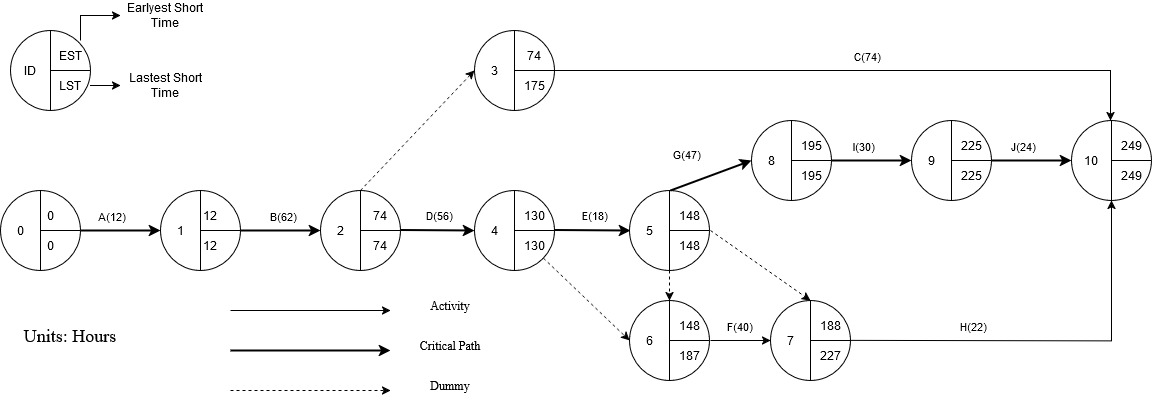
\includegraphics[width=17cm]{ActivityArrowDiagram.png} 
	\caption{Activity Arrow Diagram of ESPOLTEL HIRING MANAGER}
	\label{fig:ActivityArrowDiagram}
\end{figure}

\chapter{Static UML}
\section{Use Cases - Web Module}
\begin{figure}[H]
	\centering  \small
	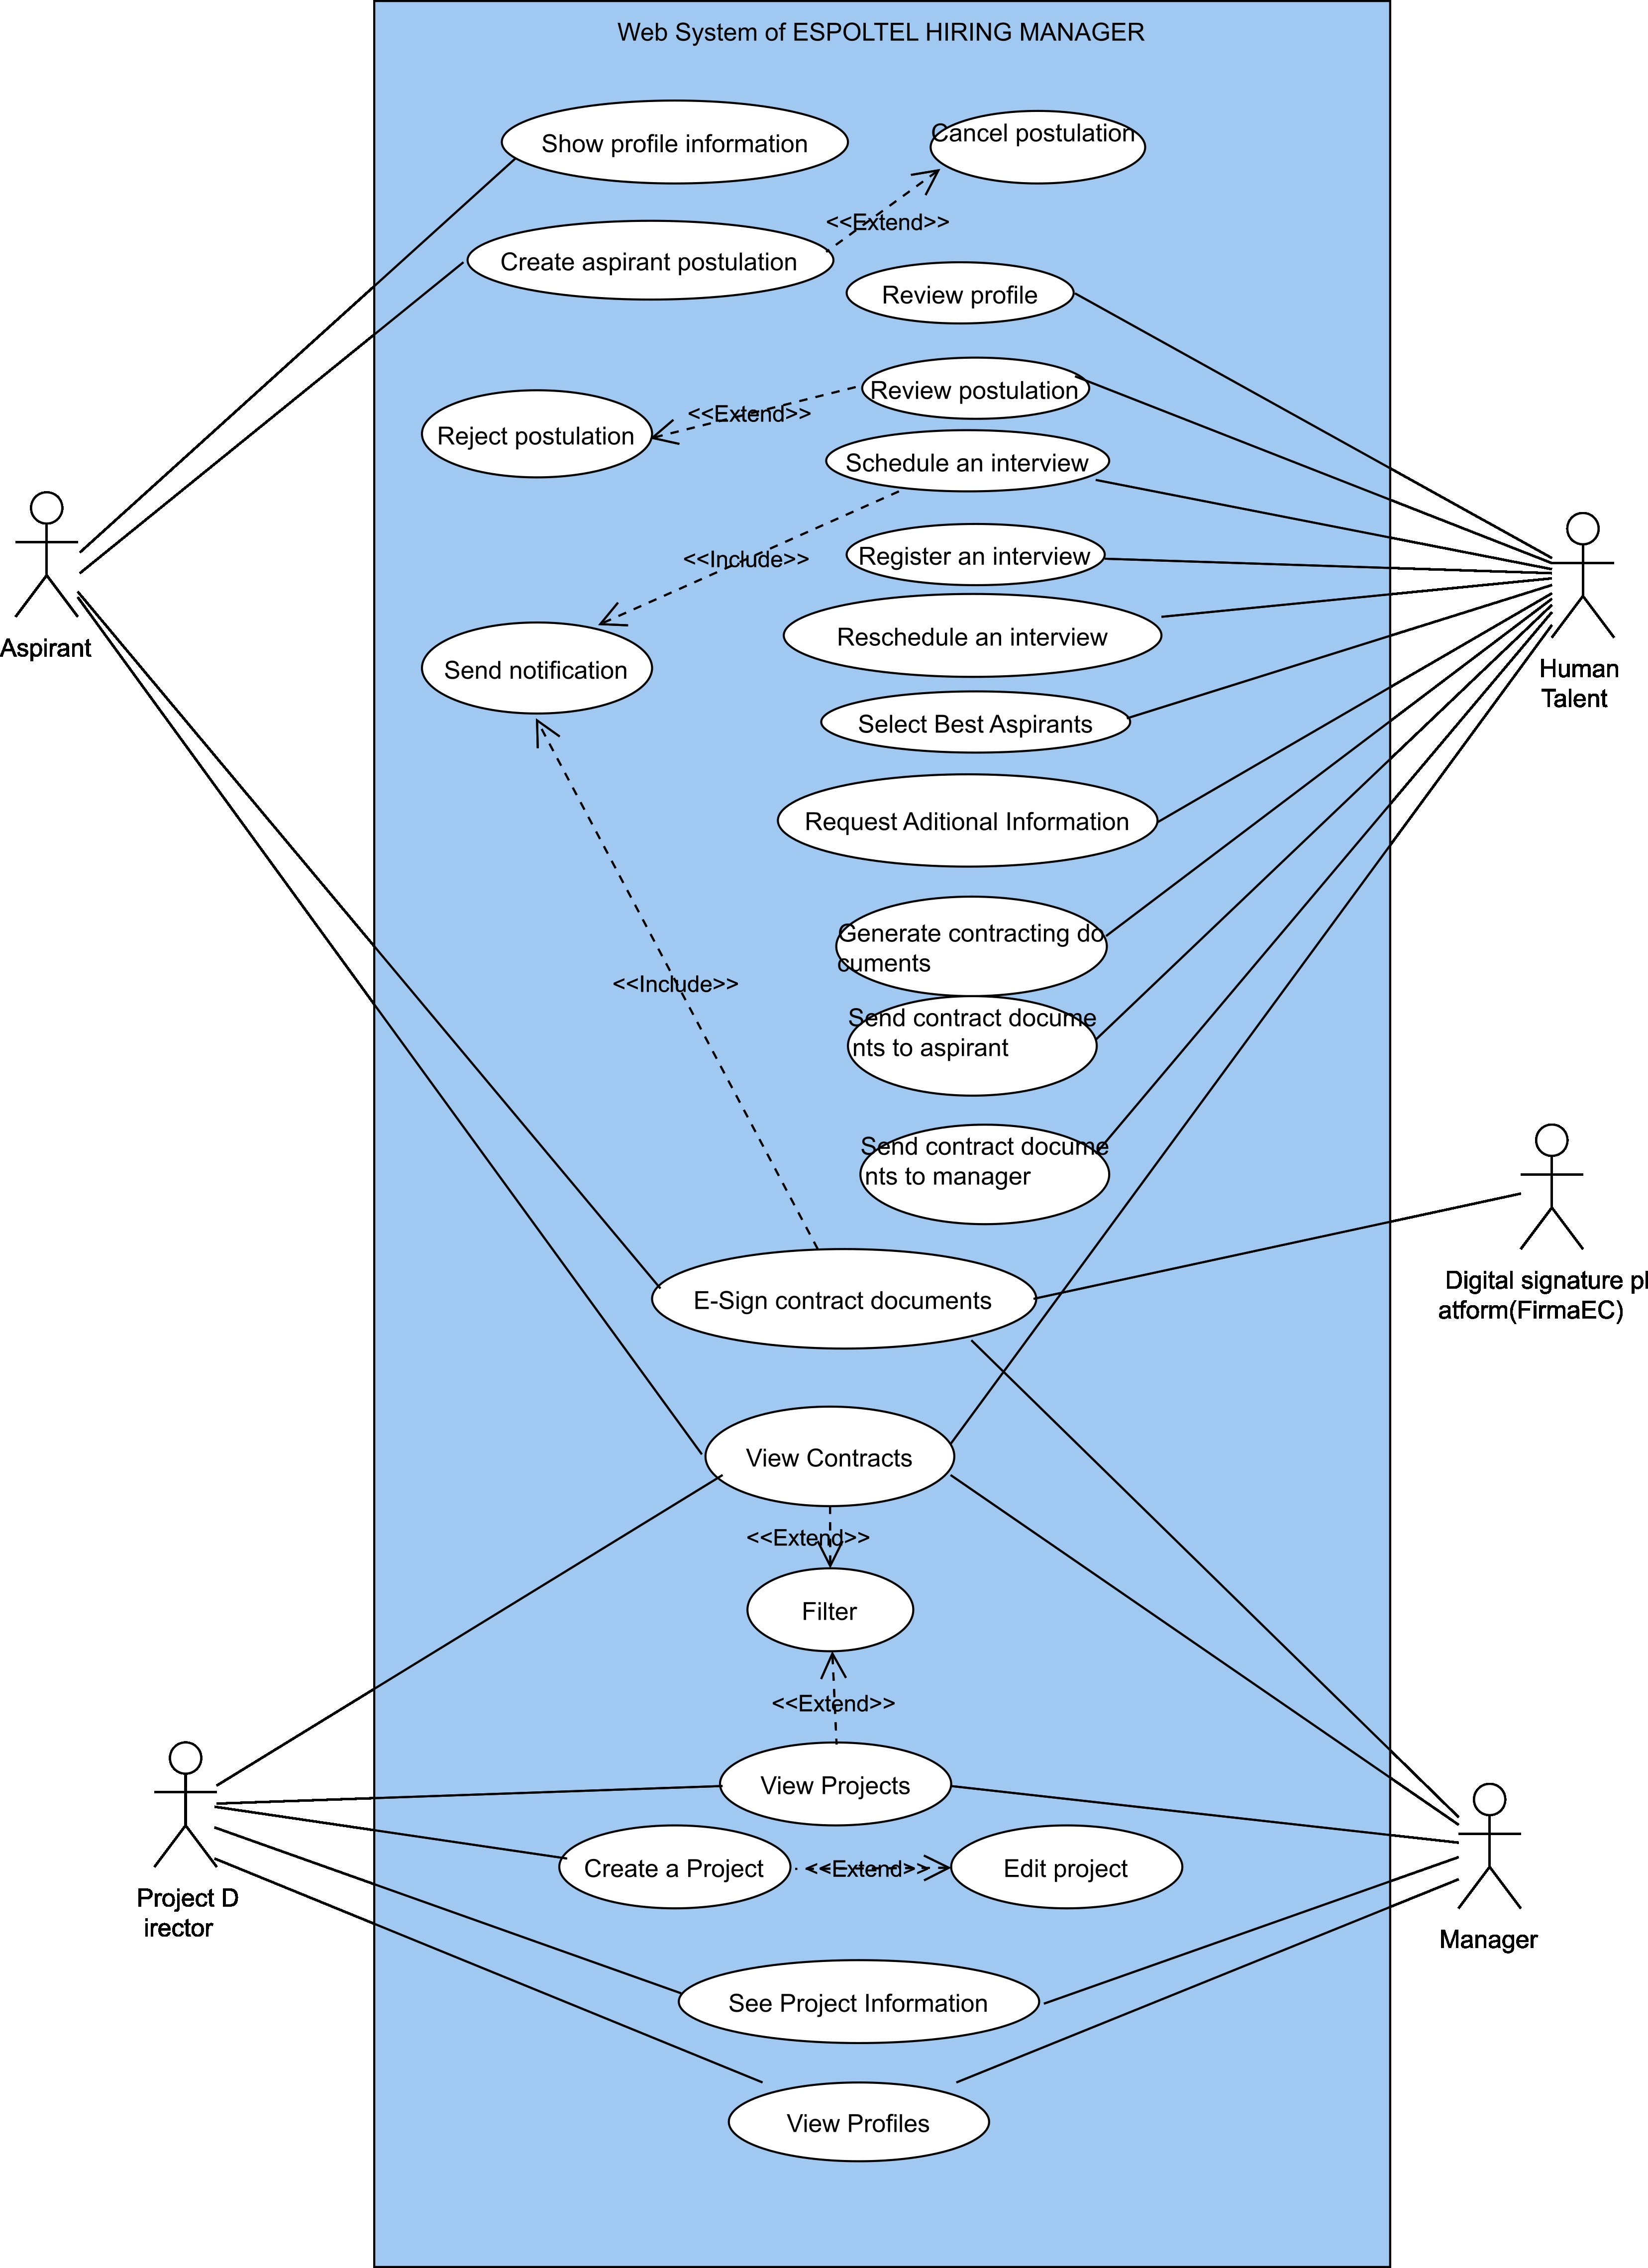
\includegraphics[width=\textwidth]{UseCases/WebUseCases.jpg} 
	\caption{Web Module Use Cases Diagram of ESPOLTEL HIRING MANAGER}
	\label{fig:WebUseCases}
\end{figure}

\begin{table}[H]
	\centering \small
	\begin{tabular}{|p{3cm}|p{10cm}|}
		\hline
		\textbf{Field} & \textbf{Description} \\ \hline
		ID & UC001 \\ \hline
		Name &  Show postulation information \\ \hline
		Created by & Jeremy Poveda \\ \hline
		Updated by & Jeremy Poveda \\ \hline
		Date creation & 8/12/24 \\ \hline
		Date last edition & 3/1/25 \\ \hline
		Description &  The system will show the aspirant the requirements, activities, and reference salary (e.g.) of the system using a code. \\ \hline
		Actors &  Aspirant \\ \hline
		Extends & Nothing \\ \hline
		Preconditions & The aspirant has his account created and is logged in, as well as the project code to which he is interested. \\ \hline
		Postconditions & The aspirant only must see the profile he/she wants to apply for with the unique code. \\ \hline
		Flow & 
		1. The aspirant enter into personnel login section. \newline
		2. The aspirant enter his credentials. \newline
		3. The system show a promt in the home page to enter a code. \newline
		4. The aspirant enters the code of the project he/she is interested in. \newline
		5. The system shows the applicant the information (Job and profile description, activities to be performed, Project name, Project description, profile requirements, and Referencial salary) of the profile he/she wants to apply for. 
		\\ \hline
		Alternative Flow &  There are no alternative flows. \\ \hline
	\end{tabular}
	\caption{Use Case Documentation - (UC001) Show Postulation Information}
	\label{table:UC001}
\end{table}
\begin{table}[H]
	\centering \small
	\begin{tabular}{|p{3cm}|p{10cm}|}
		\hline
		\textbf{Field} & \textbf{Description} \\ \hline
		ID & UC002 \\ \hline
		Name & Create aspirant postulation \\ \hline
		Created by & José Ramos \\ \hline
		Updated by & José Ramos \\ \hline
		Date creation & 8/12/24 \\ \hline
		Date last edition & 7/01/25 \\ \hline
		Description & The aspirant wants to send information in the project they are interested in. \\ \hline
		Actors & Aspirant \\ \hline
		Extends / Includes & Cancel Postulation \\ \hline
		Preconditions & 
		\begin{itemize}
			\item The aspirant has his account created and logged in, as well as the project code to which he is interested.
			\item The aspirant has a valid project code.
		\end{itemize} 
		\\ \hline
		Postconditions & The system registers the application of the aspirant. \\ \hline
		Flow & 
		    1. The aspirant logs in with his/her credentials.\newline
			2. The aspirant enters the valid code of a project.\newline
			3. The aspirant clicks on the project that appears on the screen.\newline
			4. The aspirant reads the project information.\newline
			5. The aspirant makes sure that he/she meets the minimum requirements to participate in the project.\newline
			6. The aspirant applies for the job.\newline
			7. The aspirant uploads the documents required by the system (Curriculum Vitae and copy of ID).\newline
			8. The aspirant sends the application.
		\\ \hline
		Alternative Flow & 
		\begin{enumerate}
			\item[4a.] The aspirant reads the project information. 
			\item The aspirant verifies that he or she does not meet the minimum requirements to participate in the project.
			\item The aspirant returns to the home screen.
			\item[8a.] The aspirant sends the application.
			\item The aspirant the aspirant realizes that he/she has postulate incorrectly.
			\item The aspirant cancels application.
		\end{enumerate} 
		\\ \hline
	\end{tabular}
	\caption{Use Case Documentation - (UC002) Create Aspirant Postulation}
	\label{table:UC002}
\end{table}


\begin{table}[H]
	\centering
	\begin{tabular}{|p{3cm}|p{10cm}|}
		\hline
		\textbf{Field} & \textbf{Description} \\ \hline
		ID & UC003 \\ \hline
		Name & Review profile \\ \hline
		Created by &  Jeremy Poveda \\ \hline
		Updated by & Jeremy Poveda \\ \hline
		Date creation & 8/12/24 \\ \hline
		Date last edition & 12/01/25 \\ \hline
		Description & Human Talent must review the profiles created by the director to ensure they meet the established standards and requirements. \\ \hline
		Actors & Human Talent \\ \hline
		Extends & Reject Profile \\ \hline
		Preconditions & 
		The director has created the profiles.  \newline
		The profiles have been sent to Human Talent for review.
		\\ \hline
		Postconditions & 
		Human Talent confirms that the profiles meet the required standards. \newline
		Human Talent notifies the director about the approval or rejection of the profiles.
		\\ \hline
		Flow & 
		1. Human Talent enters the profile review section. \newline
		2. Human Talent identifies the profiles created by the director. \newline
		3. Human Talent reviews the information of each profile. \newline
		4. Human Talent verifies that the profiles meet the required standards and requirements. \newline
		5. Human Talent edits in case of errors. 
		\\ \hline
		Alternative Flow & 
		\begin{enumerate}
			\item[4a.] Human Talent identifies that the profiles do meet the required standards.
			\item Human Talent accept the profile.
			\item The profile enters in 'in hiring' status.
		\end{enumerate} 
		\\ \hline
	\end{tabular}
	\caption{Use Case Documentation  - (UC003) Review Profile}
	\label{table:UC003}
\end{table}

\begin{table}[H]
	\centering
	\begin{tabular}{|p{3cm}|p{10cm}|}
		\hline
		\textbf{Field} & \textbf{Description} \\ \hline
		ID & UC004 \\ \hline
		Name & Review postulation \\ \hline
		Created by & José Ramos \\ \hline
		Updated by & José Ramos \\ \hline
		Date creation & 8/12/24 \\ \hline
		Date last edition & 12/01/25 \\ \hline
		Description & Human Talent verifies the submitted postulations, ensuring the aspirant’s data and documentation meet the required standards. \\ \hline
		Actors & Human Talent \\ \hline
		Extends & Reject Postulation \\ \hline
		Preconditions & The aspirant must have sent the form with his CV and ID. \\ \hline
		Postconditions & The aspirant is notified via email if their postulation review was successful. \\ \hline
		Flow & 
		1. Human Talent logs into the system and navigates to the postulation review section. \newline
		2. Human Talent selects a postulation to review. \newline
		3. Human Talent verifies the aspirant’s data for consistency and correctness. \newline
		4. Human Talent reviews the documentation submitted by the aspirant (CV and copy of ID). \newline
		5. Human Talent writes observations or feedback if necessary. \newline
		6. Human Talent sends a notification email to the aspirant about the result of the review. 
		\\ \hline
		Alternative Flow &  
		3a. Human Talent identifies inconsistencies in the aspirant’s data or finds incorrect documentation. \newline
		4. Human Talent writes a rejection message specifying the issues. \newline
		5. Human Talent removes the postulation from the approval process.
		\\ \hline
	\end{tabular}
	\caption{Use Case Documentation - (UC004) Review Postulation}
	\label{table:UC004}
\end{table}

\begin{table}[H]
	\centering
	\begin{tabular}{|p{3cm}|p{10cm}|}
		\hline
		\textbf{Field} & \textbf{Description} \\ \hline
		ID & UC005 \\ \hline
		Name & Schedule an interview \\ \hline
		Created by & Team 3 \\ \hline
		Updated by & Alex Vizuete \\ \hline
		Date creation & 08/01/25 \\ \hline
		Date last edition & 08/01/25 \\ \hline
		Description & Human Talent Staff need to schedule an interview for accepted aspirants by selecting a specific day and time. \\ \hline
		Actors & Human Talent \\ \hline
		Extends & None \\ \hline
		Preconditions & 
		\begin{itemize}
			\item Aspirant must be marked as accepted for the interview process.
		\end{itemize} \\ \hline
		Postconditions & 
		\begin{itemize}
			\item Aspirants are notified about the scheduled interview.
			\item Human Talent Staff can see the interview in a calendar.
		\end{itemize} \\ \hline
		Flow & 
		1. Human Talent Assistant navigates to the interviews tab. \newline
		2. The Assistant clicks on the "Create New Interview" button. \newline
		3. The Assistant selects a date using the input calendar and specifies the interview time. \newline
		4. The Assistant selects the aspirant for the interview. \newline
		5. The Assistant clicks the "Create" button. \newline
		6. The interview is scheduled and displayed in the calendar in the interviews section. \\ \hline
		Alternative Flow & None \\ \hline
	\end{tabular}
	\caption{Use Case Documentation - (UC005) Schedule an Interview}
	\label{table:UC005}
\end{table}

\begin{table}[H]
	\centering
	\begin{tabular}{|p{3cm}|p{10cm}|}
		\hline
		\textbf{Field} & \textbf{Description} \\ \hline
		ID & UC006 \\ \hline
		Name & Register an interview \\ \hline
		Created by & Jeremy Poveda \\ \hline
		Updated by & Jeremy Poveda \\ \hline
		Date creation & 9/01/25 \\ \hline
		Date last edition & 12/01/25 \\ \hline
		Description & Human Talent Staff registers the outcome of an interview by reviewing the aspirant's requirements, adding observations, and saving the result. \\ \hline
		Actors & Human Talent \\ \hline
		Extends & None \\ \hline
		Preconditions & 
		\begin{itemize}
			\item An interview must have been scheduled with the aspirant.
		\end{itemize} \\ \hline
		Postconditions & 
		\begin{itemize}
			\item The interview is marked as complete in the system.
			\item Observations and results are stored for the aspirant's record.
		\end{itemize} \\ \hline
		Flow & 
		1. Human Talent Staff navigates to the "Interviews" section. \newline
		2. The HT Staff selects the scheduled interview they wish to register. \newline
		3. The HT Staff reviews the aspirant's requirements (e.g., submitted documents, qualifications). And with the In real life interview. \newline
		4. The HT Staff writes observations about the aspirant's performance and any relevant notes. \newline
		5. The HT Staff saves the results of the interview, marking it as completed. \\ \hline
		Alternative Flow & 
		None \\ \hline
	\end{tabular}
	\caption{Use Case Documentation - (UC006) Register an Interview}
	\label{table:UC006}
\end{table}

\begin{table}[H]
	\centering
	\begin{tabular}{|p{3cm}|p{10cm}|}
		\hline
		\textbf{Field} & \textbf{Description} \\ \hline
		ID & UC007 \\ \hline
		Name & Re-schedule an interview \\ \hline
		Created by & Team 3 \\ \hline
		Updated by & Alex Vizuete \\ \hline
		Date creation & 8/01/25 \\ \hline
		Date last edition & 12/01/25 \\ \hline
		Description & Human Talent Staff handles situations where the aspirant misses the interview or cannot attend. The interview can be re-scheduled, canceled, or removed as needed. \\ \hline
		Actors & Human Talent \\ \hline
		Extends & None \\ \hline
		Preconditions & 
		\begin{itemize}
			\item The interview must have been previously scheduled.
		\end{itemize} \\ \hline
		Postconditions & 
		\begin{itemize}
			\item The interview is either re-scheduled, marked as canceled, or deleted from the system.
			\item The aspirant is notified about the change via email. 
		\end{itemize} \\ \hline
		Flow & 
		1. Human Talent Staff navigates to the "Interviews" section. \newline
		2. The HT Staff identifies the interview to be re-scheduled or canceled. \newline
		3. The HT Staff selects the option to re-schedule or cancel the interview. \newline
		4. If re-scheduling: \newline
		\hspace*{0.5cm} a. The Staff selects a new date and time for the interview. \newline
		\hspace*{0.5cm} b. The Staff notifies the aspirant about the new schedule. \newline
		5. If canceling: \newline
		\hspace*{0.5cm} b. The interview is marked as canceled or removed from the system. \newline
		6. The changes are saved in the system. \\ \hline
		Alternative Flow & 
		3a. The Staff decides to delete the interview entirely: \newline
		\hspace*{0.5cm} a. The interview is removed from the system. \newline
		\hspace*{0.5cm} b. The aspirant is notified about the removal. \\ \hline
	\end{tabular}
	\caption{Use Case Documentation - (UC007) Re-schedule an Interview}
	\label{table:UC007}
\end{table}

\begin{table}[H]
	\centering
	\begin{tabular}{|p{3cm}|p{10cm}|}
		\hline
		\textbf{Field} & \textbf{Description} \\ \hline
		ID & UC008 \\ \hline
		Name & Select Best Aspirants \\ \hline
		Created by & Jeremy Poveda \\ \hline
		Updated by & Jeremy Poveda \\ \hline
		Date creation & 8/01/25 \\ \hline
		Date last edition & 12/01/25 \\ \hline
		Description & Human Talent Staff selects the best aspirants based on interview results and the aspirant’s profile, making sure they meet the requirements for the position. \\ \hline
		Actors & Human Talent \\ \hline
		Extends & None \\ \hline
		Preconditions & 
		\begin{itemize}
			\item Aspirants must have completed their interviews.
			\item The interview results must be available and recorded.
			\item The aspirant’s profile should meet the minimum requirements of the project.
		\end{itemize} \\ \hline
		Postconditions & 
		\begin{itemize}
			\item The best aspirants are selected based on their interview results and profile compatibility.
			\item The selected aspirants are notified about their selection.
		\end{itemize} \\ \hline
		Flow & 
		1. Human Talent Staff navigates to the "Aspirants accepted" section. \newline
		2. The Staff reviews the list of aspirants who completed the interview. \newline
		3. The Staff compares the interview results and the aspirant’s profile with the requirements for the position. \newline
		4. Based on the comparison, the Staff selects the best aspirants that meet the criteria. \newline
		5. The selected aspirants are notified by email about their selection. \newline
		6. The selected aspirants are marked in the system as chosen for the next steps. \\ \hline
		Alternative Flow & 
		3a. If no aspirants meet the requirements: \newline
		\hspace*{0.5cm} a. Human Talent can decide to keep the search open for more aspirants or re-evaluate other candidates. \\ \hline
	\end{tabular}
	\caption{Use Case Documentation - (UC008) Select Best Aspirants}
	\label{table:UC008}
\end{table}

\begin{table}[H]
	\centering
	\begin{tabular}{|p{3cm}|p{10cm}|}
		\hline
		\textbf{Field} & \textbf{Description} \\ \hline
		ID & UC009 \\ \hline
		Title & Request Additional Information \\ \hline
		Author & José Ramos \\ \hline
		Updated by & José Ramos \\ \hline
		Date creation & 28/12/24 \\ \hline
		Date last edition & 12/01/2025 \\ \hline
		Description & Human Talent must ask the applicant for additional information required to continue with the hiring flow. \\ \hline
		Actors & Human Talent \\ \hline
		Extends/Includes & Send notification \\ \hline
		Preconditions & 
		\begin{itemize}
			\item The applicant must pass the interview successfully.
		\end{itemize} \\ \hline
		Postconditions & 
		\begin{itemize}
			\item The applicant receives the notification and must send the required documents to the Human Talent staff.
		\end{itemize} \\ \hline
		Flow & 
		1. Human Talent logs in. \newline
		2. Human Talent goes to the “Recruitment Forms” section. \newline
		3. Human Talent selects the project they want to review. \newline
		4. Human Talent selects one of the aspirants. \newline
		5. Human Talent checks the correct documents with the checkbox. \newline
		6. Human Talent presses the button to send the review. \newline
		7. Human Talent writes a comment where they ask for the required documents. \newline
		8. Human Talent sends the notification to the aspirants. \\ \hline
		Alternative Flow & None \\ \hline
	\end{tabular}
	\caption{Use Case Documentation - (UC009) Request Additional Information}
	\label{table:UC009}
\end{table}

\begin{table}[H]
	\centering
	\begin{tabular}{|p{3cm}|p{10cm}|}
		\hline
		\textbf{Field} & \textbf{Description} \\ \hline
		ID & UC010 \\ \hline
		Title & Generate Contracting Document \\ \hline
		Author & Jeremy Poveda \\ \hline
		Updated by & Jeremy Poveda \\ \hline
		Date creation & 29/12/24 \\ \hline
		Date last edition & 12/01/2025 \\ \hline
		Description & 
		Human Talent uses the Recruitment Forms from the previous use case and a pre-created Word document template to generate a contracting document by merging the form data with the template. The corresponding data will be matched with placeholders in the Word document. \\ \hline
		Actors & Human Talent \\ \hline
		Extends/Includes & None\\ \hline
		Preconditions & 
		\begin{itemize}
			\item The applicant must have successfully passed the interview.
			\item The required documents must have been received and reviewed.
			\item A pre-created Word template for the contracting document exists.
		\end{itemize} \\ \hline
		Postconditions & 
		\begin{itemize}
			\item A contracting document is generated with the applicant’s data from the Recruitment Form.
			\item The generated document is saved and can be sent to the aspirant.
		\end{itemize} \\ \hline
		Flow & 
		1. Human Talent logs in. \newline
		2. Human Talent goes to the “Generación de documentos” section. \newline
		3. Human Talent selects the recruitment form of the applicant they wish to generate the document for. \newline
		4. Human Talent uploads the pre-created Word document template. \newline
		5. Human Talent matches the corresponding fields in the form to the placeholders in the Word template. \newline
		6. Human Talent generates the document by merging the form data with the template. \newline
		7. Human Talent reviews the generated document. \newline
		8. Human Talent saves the document for future use or sends it to the applicant. \\ \hline
		Alternative Flow & 
		\begin{itemize}
			\item  If an error occurs while merging the form data with the template, Human Talent can attempt the process again or manually resolve the issue.
		\end{itemize} \\ \hline
	\end{tabular}
	\caption{Use Case Documentation - (UC010) Generate Contracting Document}
	\label{table:UC010}
\end{table}

\begin{table}[H]
	\centering
	\begin{tabular}{|p{3cm}|p{10cm}|}
		\hline
		\textbf{Field} & \textbf{Description} \\ \hline
		ID & UC011 \\ \hline
		Title & Send Contracting Document to aspirant\\ \hline
		Author & Jeremy Poveda\\ \hline
		Updated by &  Jeremy Poveda \\ \hline
		Date creation & 29/12/24 \\ \hline
		Date last edition & 12/01/2025 \\ \hline
		Description & 
		Human Talent sends the generated contracting documents to the aspirant for his/her esign. \\ \hline
		Actors & Human Talent \\ \hline
		Extends/Includes & None \\ \hline
		Preconditions & 
		\begin{itemize}
			\item The contracting document must have been generated and reviewed.
		\end{itemize} \\ \hline
		Postconditions & 
		\begin{itemize}
			\item The applicant receives the document ready for e-signing.
		\end{itemize} \\ \hline
		Flow & 
		1. Human Talent logs in. \newline
		2. Human Talent goes to the “Generación de documentos" section. \newline
		3. Human Talent selects the aspirant with the document to be sent. \newline
		4. Human Talent clicks to send to aspirant. \newline
		5. Human Talent sends the document. \\ \hline
		Alternative Flow & 
		None\\ \hline
	\end{tabular}
	\caption{Use Case Documentation - (UC011) Send Contracting Document to aspirant}
	\label{table:UC011}
\end{table}

\begin{table}[H]
	\centering
	\begin{tabular}{|p{3cm}|p{10cm}|}
		\hline
		\textbf{Field} & \textbf{Description} \\ \hline
		ID & UC012 \\ \hline
		Title & Send Contracting Documents to Manager \\ \hline
		Author & Jeremy Poveda\\ \hline
		Updated by & Jeremy Poveda \\ \hline
		Date creation & 29/12/24 \\ \hline
		Date last edition & 12/01/2025 \\ \hline
		Description & 
		Human Talent sends the generated contracting documents for multiple applicants to the manager for review. \\ \hline
		Actors & Human Talent \\ \hline
		Extends/Includes & None \\ \hline
		Preconditions & 
		\begin{itemize}
			\item The contracting documents must have been generated and reviewed for the applicants.
		\end{itemize} \\ \hline
		Postconditions & 
		\begin{itemize}
			\item The manager receives the documents for review and final approval.
		\end{itemize} \\ \hline
		Flow & 
		1. Human Talent logs in. \newline
		2. Human Talent goes to the “Generación de documentos” section. \newline
		3. Human Talent selects the applicants whose documents need to be sent. \newline
		4. Human Talent clicks the option to send selected documents to the manager. \newline
		5. Verify the esign of the aspirant.\newline
		6. Human Talent sends the documents. If they are correctly esigned. \\ \hline
		Alternative Flow & 
		5a. The esign it's incorrect. \newline
		1. Human talent asks the aspirant to e-sign again.
		\\ \hline
	\end{tabular}
	\caption{Use Case Documentation - (UC012) Send Contracting Documents to Manager}
	\label{table:UC012}
\end{table}

\begin{table}[H]
	\centering
	\begin{tabular}{|p{3cm}|p{10cm}|}
		\hline
		\textbf{Field} & \textbf{Description} \\ \hline
		ID & UC013 \\ \hline
		Title & E-sign Contract Documents \\ \hline
		Author & Diego Flores \\ \hline
		Updated by & Diego Flores \\ \hline
		Date creation & 23/12/24 \\ \hline
		Date last edition & 12/1/25 \\ \hline
		Description & 
		After the aspirant sends the personal data requested by human talent, they need to sign the respective contract to complete the hiring process. \\ \hline
		Actors & Aspirant \\ \hline
		Extends/Includes & None \\ \hline
		Preconditions & 
		\begin{itemize}
			\item The aspirant submits preliminary documents (resume and ID copy).
			\item Human Resources approves the preliminary documents and schedules an interview.
			\item The aspirant must have attended the interview.
			\item The aspirant must be accepted by Human Resources during the candidate acceptance process.
			\item The aspirant submits the required documents that are requested.
			\item Human Resources ensures the validity of the submitted documents.
			\item The aspirant is notified to sign the contract to complete the hiring process.
		\end{itemize} \\ \hline
		Postconditions & 
		\begin{itemize}
			\item The aspirant is notified that they have been hired for the project they initially applied for.
		\end{itemize} \\ \hline
		Flow & 
		1. The aspirant gets notified to sign the contract through the app. \newline
		2. The aspirant logs into their account. \newline
		3. The aspirant goes to the contract module. \newline
		4. The aspirant selects the contract assigned by Human Talent. \newline
		5. The aspirant signs the contract. \\ \hline
		Alternative Flow & 
		1. If the user forgets to sign the contract: \newline
		2. Five days after Human Talent has sent the contract, the aspirant is notified again to sign it. \\ \hline
	\end{tabular}
	\caption{Use Case Documentation - (UC013) E-sign Contract Documents}
	\label{table:UC013}
\end{table}

\begin{table}[H]
	\centering
	\begin{tabular}{|p{3cm}|p{10cm}|}
		\hline
		\textbf{Field} & \textbf{Description} \\ \hline
		ID & UC014 \\ \hline
		Title & View contracts \\ \hline
		Author & Diego Flores \\ \hline
		Updated by & Diego Flores \\ \hline
		Date creation & 16/12/24 \\ \hline
		Date last edition & 3/1/25 \\ \hline
		Description & 
		The manager through the mobile application will be able to find the applicants whose contracts are available to sign. \\ \hline
		Actors & Manager \\ \hline
		Extends & 
		\begin{itemize}
			\item Filter2
		\end{itemize} \\ \hline
		Preconditions & 
		\begin{itemize}
			\item The manager must have logged into their account
		\end{itemize} \\ \hline
		Postconditions & 
		None \\ \hline
		Flow & 
		1. The manager logs into their account from the mobile application. \newline
		2. The manager heads over to the "view contracts" module. \newline
		3. The manager filters the applicant's contract to review the number of pending contracts to be signed. \\ \hline
		Alternative Flow & 
		\begin{itemize}
			\item Filter applicant's contract by project.
			\item Filter applicant's contract by Employment Relationship.
		\end{itemize} \\ \hline
	\end{tabular}
	\caption{Use Case Documentation - (UC014) View Contracts}
	\label{table:UC014}
\end{table}

\begin{table}[H]
	\centering
	\begin{tabular}{|p{3cm}|p{10cm}|}
		\hline
		\textbf{Field} & \textbf{Description} \\ \hline
		ID & UC015 \\ \hline
		Title & View Projects \\ \hline
		Author & José Ramos \\ \hline
		Updated by & José Ramos \\ \hline
		Date creation & 13/01/25 \\ \hline
		Date last edition & 16/01/25 \\ \hline
		Description & 
		The manager or project director will be able to see all the projects he or she is associated with, along with their description, staff, start and end dates, and project status. \\ \hline
		Actors & Manager, Director\\ \hline
		Extends & None \\ \hline
		Preconditions & 
		\begin{itemize}
			\item The manager/director must have an account in the system and must have previously created projects.
		\end{itemize} \\ \hline
		Postconditions & 
		\begin{itemize}
			\item The manager/director ensures the flow of the application process for his projects and can act depending on the status of the project.
		\end{itemize} \\ \hline
		Flow & 
		1. The manager/director  enters the internal staff section. \newline
		2. The manager/director  selects the corresponding role from the options. \newline
		3. The manager/director  logs into the system with his credentials. \newline
		4. The manager/director  selects the "my projects" section. \newline
		5. The manager/director  sees the list of projects he has previously created to which he is linked. \\ \hline
		Alternative Flow & 
		None \\ \hline
	\end{tabular}
	\caption{Use Case Documentation - (UC015) View Projects}
	\label{table:UC015}
\end{table}

\begin{table}[H]
	\centering
	\begin{tabular}{|p{3cm}|p{10cm}|}
		\hline
		\textbf{Field} & \textbf{Description} \\ \hline
		ID & UC016 \\ \hline
		Title & See Project’s Information \\ \hline
		Author & Diego Flores  \\ \hline
		Updated by & Diego Flores \\ \hline
		Date creation & 08/01/25 \\ \hline
		Date last edition & 08/01/25 \\ \hline
		Description & 
		“See project’s details” is a system feature that allows the project director to review details of his/her projects, such as the number of applicants hired and their personal data, and the job application status of those applicants who haven’t been hired. \\ \hline
		Actors & Project Director \\ \hline
		Extends & Edit project \\ \hline
		Preconditions & 
		\begin{itemize}
			\item The director must have selected a project that’s displayed in the project’s table list.
		\end{itemize} \\ \hline
		Postconditions & 
		\begin{itemize}
			\item The project director will be able to see detailed information about applicants and their job application status.
		\end{itemize} \\ \hline
		Flow & 
		1. The director logs in to his/her account. \newline
		2. The director clicks on “Mis proyectos.” \newline
		3. The director clicks on any of the projects in the project’s table list. \\ \hline
		Alternative Flow & 
		\textbf{Project director edits a project:} \newline
		1. The director logs in to his/her account. \newline
		2. The director clicks on “Mis proyectos.” \newline
		3. The director clicks on any of the projects in the project’s table list. \newline
		4. The director clicks on “Estado de perfiles.” \newline
		5. The director will be able to change the job project’s details such as the project’s name, description, and project duration. The director will also be able to add a new profile vacancy. \newline
		\textbf{Project director clicks on “Estado de perfiles”:} \newline
		1. The director logs in to his/her account. \newline
		2. The director clicks on “Mis proyectos.” \newline
		3. The director clicks on any of the projects in the project’s table list. \newline
		4. The director clicks on “Estado de perfiles.” \newline
		5. The project director will be able to review the details of the aspirants, including name, ID, and postulation status. \\ \hline
	\end{tabular}
	\caption{Use Case Documentation - (UC016) See Project’s Information}
	\label{table:UC016}
\end{table}
\begin{table}[H]
	\centering
	\begin{tabular}{|p{3cm}|p{10cm}|}
		\hline
		\textbf{Field} & \textbf{Description} \\ \hline
		ID & UC017 \\ \hline
		Title & See Profiles \\ \hline
		Author & Jeremy Poveda \\ \hline
		Updated by & Jeremy Poveda\\ \hline
		Date creation & 10/01/25 \\ \hline
		Date last edition & 16/01/25 \\ \hline
		Description & 
		This feature allows the project manager or project director to filter applicants by project and view their application status for each profile. \\ \hline
		Actors & Project Manager, Project Director \\ \hline
		Extends & None \\ \hline
		Preconditions & 
		\begin{itemize}
			\item The manager or project director must be logged into the system.
			\item The manager or project director must have at least one project with profiles and applicants associated.
		\end{itemize} \\ \hline
		Postconditions & 
		\begin{itemize}
			\item The manager or project director will be able to filter applicants by project and review the status of their applications.
		\end{itemize} \\ \hline
		Flow & 
		1. The manager or project director logs into the system. \newline
		2. The manager or project director navigates to the “Profiles” section. \newline
		3. The manager or project director applies a filter to select the desired project. \newline
		4. The system displays a list of applicants for the selected project. \newline
		5. The manager or project director reviews the postulation status for each applicant profile (e.g., accepted, pending contract sign, completed). \\ \hline
		Alternative Flow & 
		\textbf{Filter applicants by status:} \newline
		1. The manager or project director logs into the system. \newline
		2. The manager or project director navigates to the “Perfiles” section. \newline
		3. The manager or project director applies a filter to view applicants based on their application status (e.g., pending, accepted, rejected). \\ \hline
	\end{tabular}
	\caption{Use Case Documentation - (UC017) See Profiles }
	\label{table:UC017}
\end{table}



\section{Use Cases - Mobile Module}
\begin{figure}[H]
	\centering  \small
	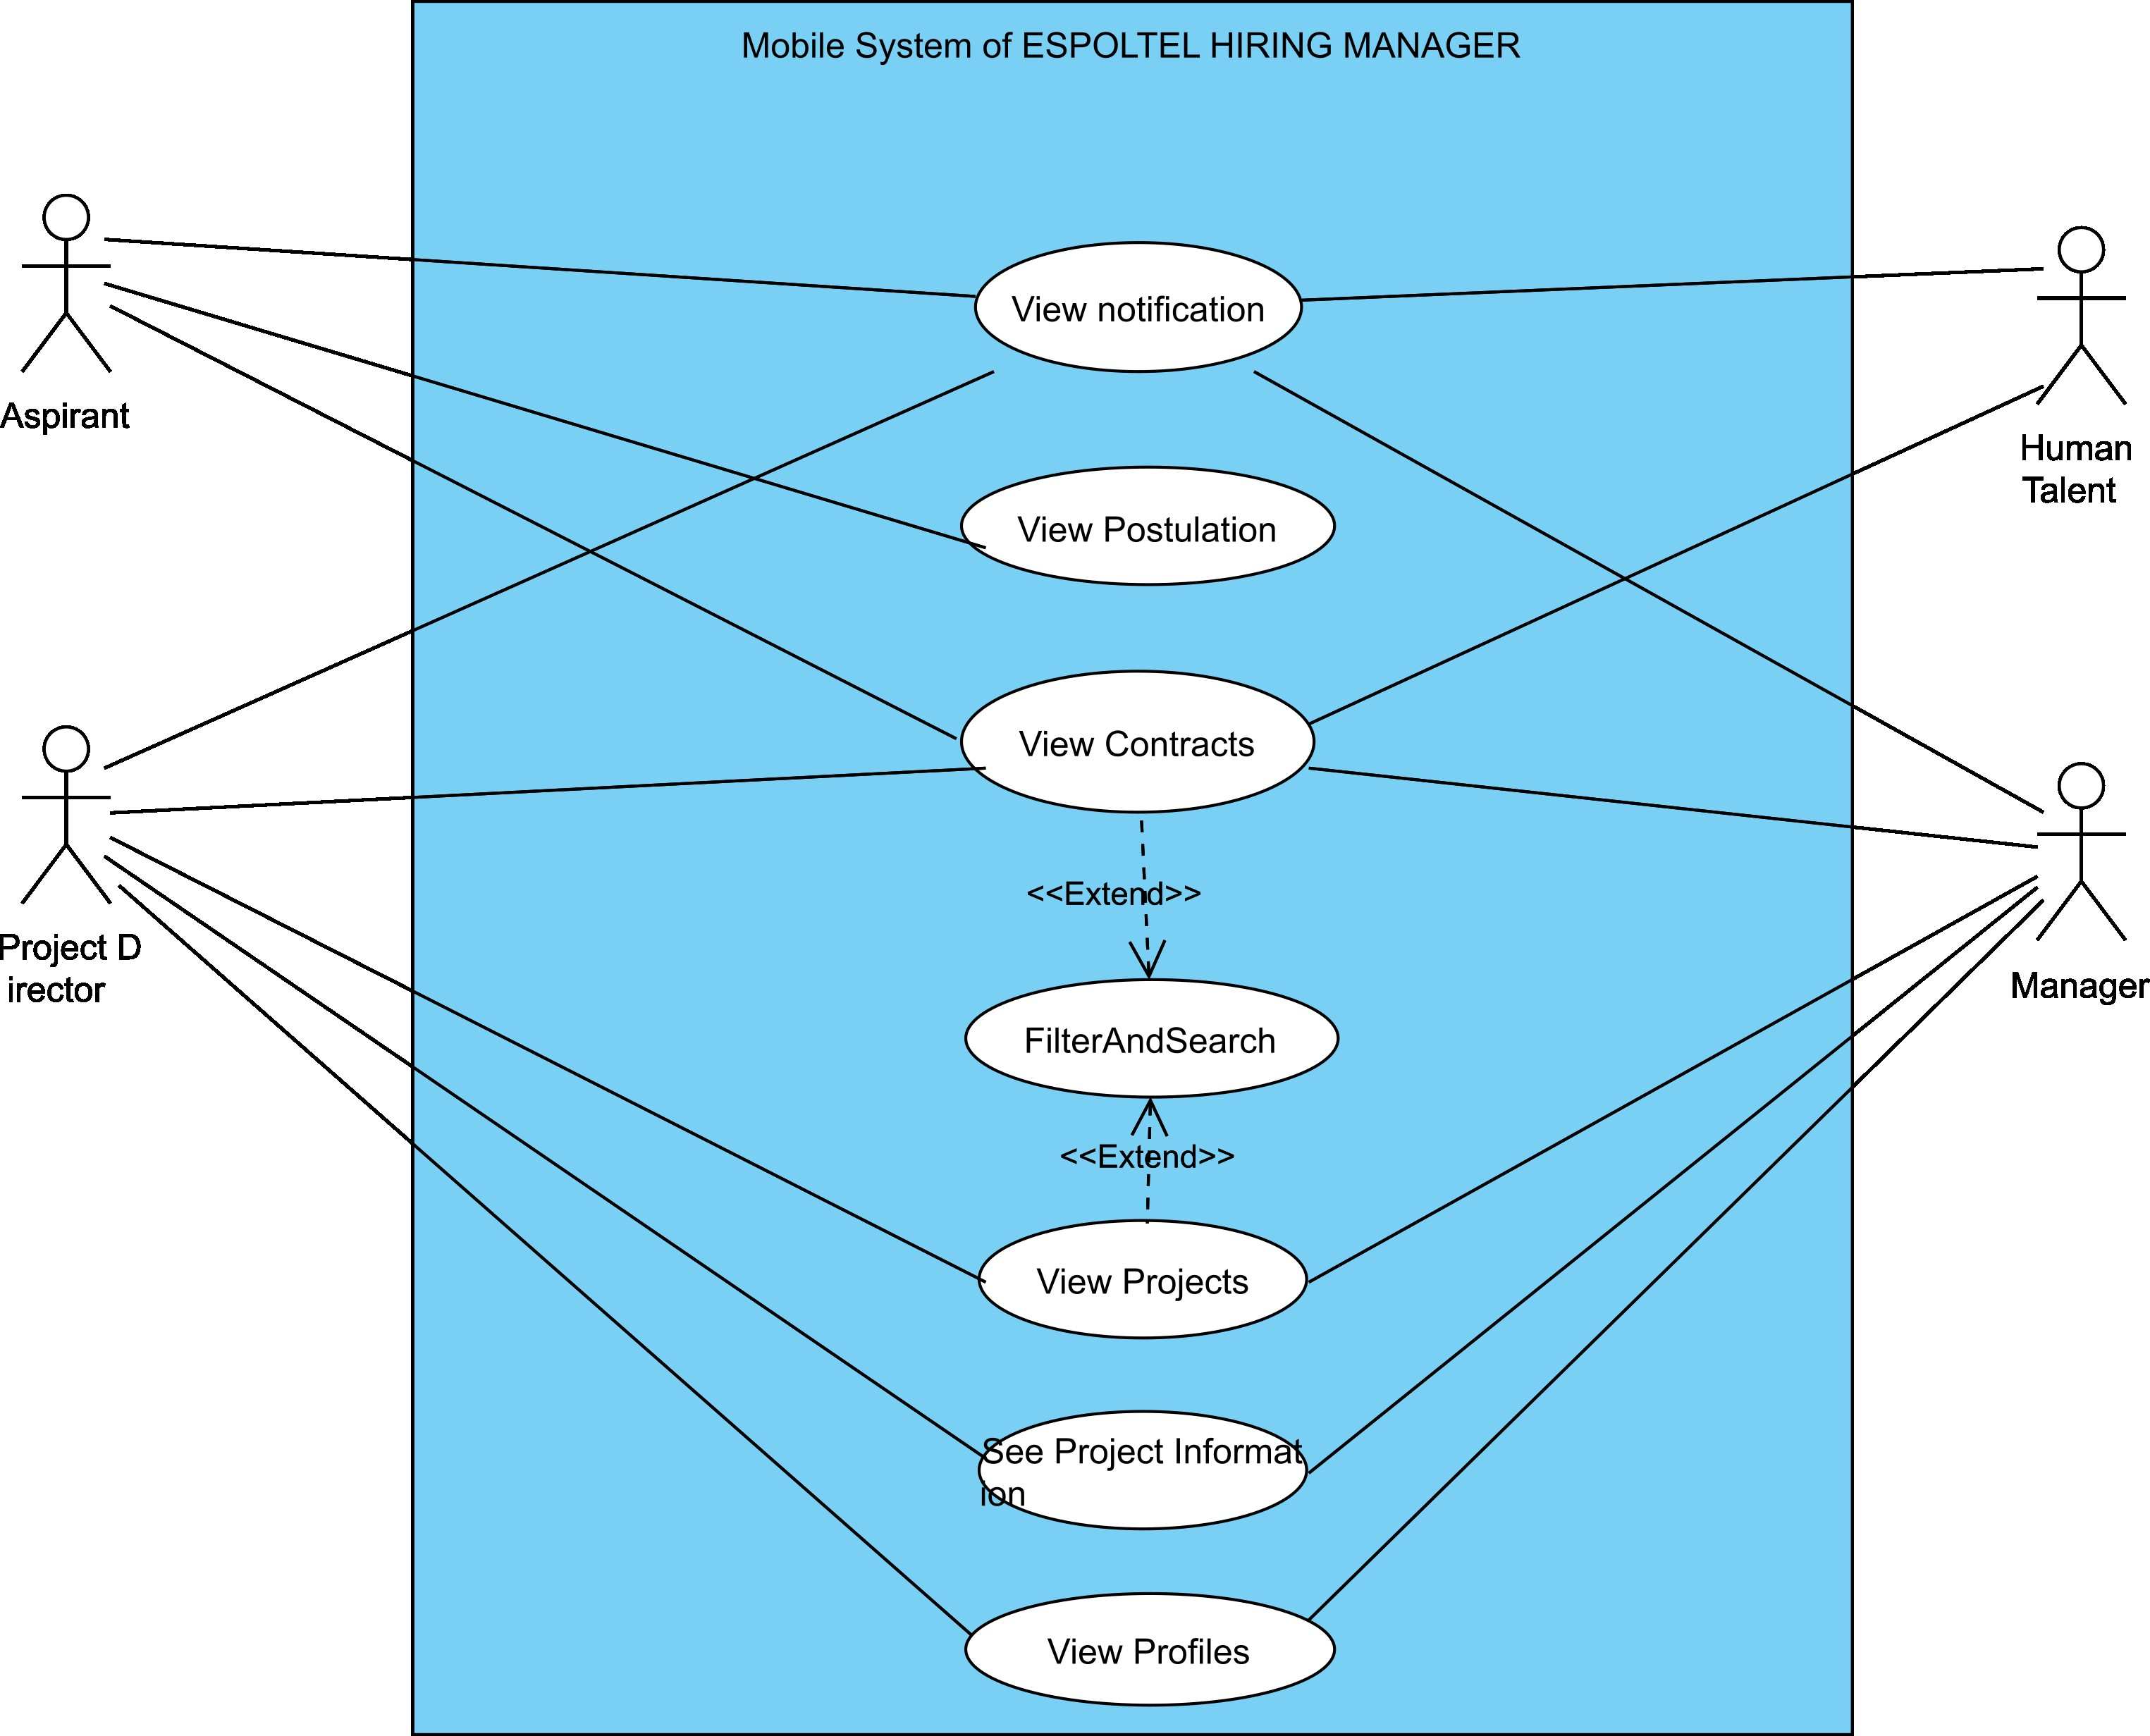
\includegraphics[width=\textwidth]{UseCases/MobileUseCases.jpg} 
	\caption{Mobile Module Use Cases Diagram of ESPOLTEL HIRING MANAGER}
	\label{fig:MobileUseCases}
\end{figure}

\begin{table}[H]
	\centering
	\begin{tabular}{|p{3cm}|p{10cm}|}
		\hline
		\textbf{Field} & \textbf{Description} \\ \hline
		ID & UC018 \\ \hline
		Title & View Notifications on Mobile \\ \hline
		Author & Jeremy Poveda \\ \hline
		Updated by & Jeremy Poveda \\ \hline
		Date creation & 8/01/25 \\ \hline
		Date last edition & 17/01/25 \\ \hline
		Description & 
		This feature allows any user of ESPOLTEL HIRING MANAGER (Director, Aspirant, Manager, Human Talent) to receive notifications on their mobile device about important updates regarding the hiring process and project management. \\ \hline
		Actors & Director, Aspirant, Manager, Human Talent \\ \hline
		Extends & None \\ \hline
		Preconditions & 
		\begin{itemize}
			\item The user must have an account in the system.
			\item The user must have a mobile device with the ESPOLTEL HIRING MANAGER app installed.
			\item The user must have enabled notifications for the app.
		\end{itemize} \\ \hline
		Postconditions & 
		\begin{itemize}
			\item The user will receive real-time notifications about relevant actions or updates in the hiring process and project status.
		\end{itemize} \\ \hline
		Flow & 
		1. The user configures their mobile device to receive notifications from the ESPOLTEL HIRING MANAGER app. \newline
		2. The system detects relevant events related to hiring or projects. \newline
		3. The system sends a notification to the user's mobile device, informing them about events such as:
		\begin{itemize}
			\item A new candidate has been accepted or rejected.
			\item A document has been requested or received.
			\item A contract is ready for signature.
			\item A project has an important update.
			\item The status of an applicant's postulation has changed.
		\end{itemize}
		4. The user receives the notification and can view additional details via the mobile app. \\ \hline
		Alternative Flow & 
		\textbf{If the user has notifications disabled:} \newline
		1. The system will notify the user to enable notifications in their device settings. \newline
		2. Once enabled, the user will begin receiving notifications as described in the main flow. \\ \hline
	\end{tabular}
	\caption{Use Case Documentation - (UC018) Receive Notifications on Mobile}
	\label{table:UC018}
\end{table}

\begin{table}[H]
	\centering \small
	\begin{tabular}{|p{3cm}|p{10cm}|}
		\hline
		\textbf{Field} & \textbf{Description} \\ \hline
		ID & UC019 \\ \hline
		Name & View application status on mobile \\ \hline
		Created by & Jeremy Poveda \\ \hline
		Updated by & Jeremy Poveda \\ \hline
		Date creation & 8/01/25 \\ \hline
		Date last edition & 17/01/25 \\ \hline
		Description & The system allows the aspirant to view the status of their application (e.g., accepted, pending, rejected) for a specific project, using a unique code, optimized for mobile devices. \\ \hline
		Actors & Aspirant \\ \hline
		Extends & Nothing \\ \hline
		Preconditions & The aspirant has an account created and is logged in, as well as the project code they are interested in. The system must be optimized for mobile use. \\ \hline
		Postconditions & The aspirant will be able to see the status of their application for the selected project, with the unique code, on their mobile device. \\ \hline
		Flow & 
		1. The aspirant opens the ESPOLTEL HIRING MANAGER app on their mobile device. \newline
		2. The aspirant enters their credentials in the login section. \newline
		5. The system displays the status (e.g., accepted, pending, rejected) of the profile they applied for, optimized for mobile viewing. 
		\\ \hline
		Alternative Flow & There are no alternative flows. \\ \hline
	\end{tabular}
	\caption{Use Case Documentation - (UC019) View Application Status on Mobile}
	\label{table:UC019}
\end{table}

\begin{table}[H]
	\centering
	\begin{tabular}{|p{3cm}|p{10cm}|}
		\hline
		\textbf{Field} & \textbf{Description} \\ \hline
		ID & UC020 \\ \hline
		Title & View contracts on mobile \\ \hline
		Author & Jeremy Poveda \\ \hline
		Updated by & Jeremy Poveda \\ \hline
		Date creation & 8/12/24 \\ \hline
		Date last edition & 16/12/24 \\ \hline
		Description & 
		The manager, through the mobile application, will be able to find the applicants whose contracts are available to sign and review them easily on their mobile device. \\ \hline
		Actors & Manager \\ \hline
		Extends & 
		\begin{itemize}
			\item Filter
		\end{itemize} \\ \hline
		Preconditions & 
		\begin{itemize}
			\item The manager must have logged into their account on the mobile application.
		\end{itemize} \\ \hline
		Postconditions & 
		None \\ \hline
		Flow & 
		1. The manager opens the ESPOLTEL HIRING MANAGER mobile application and logs into their account. \newline
		2. The manager navigates to the "View contracts" module. \newline
		3. The manager applies filters to view and review the applicants' contracts available to be signed on their mobile device. \\ \hline
		Alternative Flow & 
		\begin{itemize}
			\item Filter applicants' contracts by project.
			\item Filter applicants' contracts by Employment Relationship.
		\end{itemize} \\ \hline
	\end{tabular}
	\caption{Use Case Documentation - (UC020) View Contracts on Mobile}
	\label{table:UC020}
\end{table}

\begin{table}[H]
	\centering
	\begin{tabular}{|p{3cm}|p{10cm}|}
		\hline
		\textbf{Field} & \textbf{Description} \\ \hline
		ID & UC021 \\ \hline
		Title & View Projects on Mobile \\ \hline
		Author & José Ramos \\ \hline
		Updated by & Jeremy Poveda\\ \hline
		Date creation & 8/01/25 \\ \hline
		Date last edition & 16/01/25 \\ \hline
		Description & 
		The manager or project director will be able to view all the projects they are associated with, along with their descriptions, staff, start and end dates, and project status, directly from their mobile device. \\ \hline
		Actors & Manager, Director \\ \hline
		Extends & None \\ \hline
		Preconditions & 
		\begin{itemize}
			\item The manager or director must have an account in the system and must have previously created projects.
		\end{itemize} \\ \hline
		Postconditions & 
		\begin{itemize}
			\item The manager or director will be able to monitor the application process for their projects and take necessary actions based on the project status, directly from their mobile device.
		\end{itemize} \\ \hline
		Flow & 
		1. The manager or director opens the ESPOLTEL HIRING MANAGER mobile app. \newline
		2. The manager or director navigates to the "My Projects" section. \newline
		3. The manager or director logs into the system using their credentials. \newline
		4. The system displays a list of projects that the manager or director is associated with, showing project descriptions, staff, start and end dates, and project status. \\ \hline
		Alternative Flow & 
		None \\ \hline
	\end{tabular}
	\caption{Use Case Documentation - (UC021) View Projects on Mobile}
	\label{table:UC021}
\end{table}

\begin{table}[H]
	\centering
	\begin{tabular}{|p{3cm}|p{10cm}|}
		\hline
		\textbf{Field} & \textbf{Description} \\ \hline
		ID & UC022 \\ \hline
		Title & See Project’s Information on Mobile \\ \hline
		Author & Diego Flores \\ \hline
		Updated by & Diego Flores \\ \hline
		Date creation & 08/01/25 \\ \hline
		Date last edition & 08/01/25 \\ \hline
		Description & 
		“See project’s details” is a system feature that allows the project director to review details of his/her projects from the mobile app, such as the number of applicants hired and their personal data, and the job application status of those applicants who haven’t been hired. \\ \hline
		Actors & Project Director \\ \hline
		Extends & Edit project \\ \hline
		Preconditions & 
		\begin{itemize}
			\item The director must have selected a project displayed in the project’s list on the mobile app.
		\end{itemize} \\ \hline
		Postconditions & 
		\begin{itemize}
			\item The project director will be able to see detailed information about applicants and their job application status directly from their mobile device.
		\end{itemize} \\ \hline
		Flow & 
		1. The director opens the mobile app and logs into their account. \newline
		2. The director navigates to the "My Projects" section in the app. \newline
		3. The director selects a project from the list of their projects displayed in the app. \\ \hline
		Alternative Flow & 
		\textbf{Project director edits a project:} \newline
		1. The director opens the mobile app and logs into their account. \newline
		2. The director navigates to the "My Projects" section in the app. \newline
		3. The director selects a project from the list of their projects. \newline
		4. The director taps on "Profile Status." \newline
		5. The director can edit project details such as name, description, and project duration, and add new profile vacancies. \newline
		\textbf{Project director clicks on “Profile Status”:} \newline
		1. The director opens the mobile app and logs into their account. \newline
		2. The director navigates to the "My Projects" section. \newline
		3. The director selects a project from the list. \newline
		4. The director taps on "Profile Status." \newline
		5. The director can review the applicants’ details including name, ID, and postulation status. \\ \hline
	\end{tabular}
	\caption{Use Case Documentation - (UC022) See Project’s Information on Mobile}
	\label{table:UC022}
\end{table}

\begin{table}[H]
	\centering
	\begin{tabular}{|p{3cm}|p{10cm}|}
		\hline
		\textbf{Field} & \textbf{Description} \\ \hline
		ID & UC023 \\ \hline
		Title & See Profiles on Mobile \\ \hline
		Author & Jeremy Poveda \\ \hline
		Updated by & Jeremy Poveda \\ \hline
		Date creation & 8/01/25 \\ \hline
		Date last edition & 16/01/25 \\ \hline
		Description & 
		This feature allows the project manager or project director to filter applicants by project and view their application status for each profile directly from their mobile device. \\ \hline
		Actors & Project Manager, Project Director \\ \hline
		Extends & None \\ \hline
		Preconditions & 
		\begin{itemize}
			\item The manager or project director must be logged into the system via the mobile app.
			\item The manager or project director must have at least one project with profiles and applicants associated.
		\end{itemize} \\ \hline
		Postconditions & 
		\begin{itemize}
			\item The manager or project director will be able to filter applicants by project and review the status of their applications directly from their mobile device.
		\end{itemize} \\ \hline
		Flow & 
		1. The manager or project director opens the mobile app and logs into the system. \newline
		2. The manager or project director navigates to the “Profiles” section in the app. \newline
		3. The manager or project director applies a filter to select the desired project from the list. \newline
		4. The system displays a list of applicants for the selected project. \newline
		5. The manager or project director reviews the postulation status for each applicant profile (e.g., accepted, pending contract sign, completed). \\ \hline
		Alternative Flow & 
		\textbf{Filter applicants by status on mobile:} \newline
		1. The manager or project director opens the mobile app and logs into the system. \newline
		2. The manager or project director navigates to the “Perfiles” section in the app. \newline
		3. The manager or project director applies a filter to view applicants based on their application status (e.g., pending, accepted, rejected). \\ \hline
	\end{tabular}
	\caption{Use Case Documentation - (UC023) See Profiles on Mobile}
	\label{table:UC023}
\end{table}

\section{Class Diagram - Web Module}
\begin{figure}[H]
	\centering  \small
	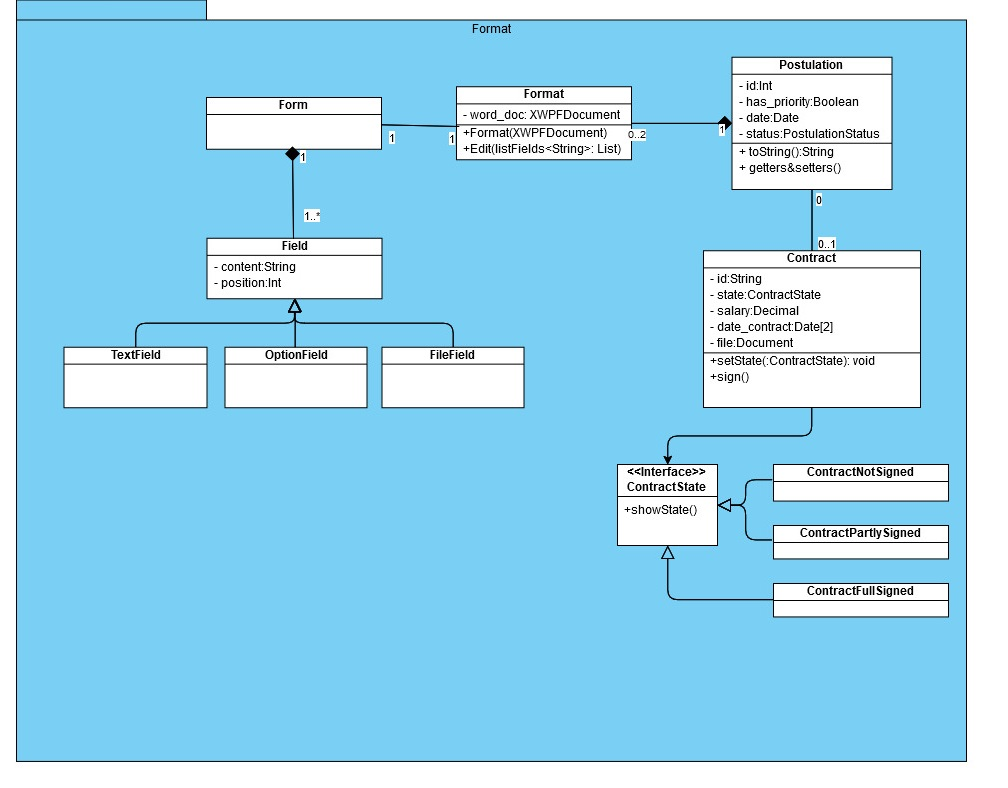
\includegraphics[width=\textwidth]{DC/DC1.jpg} 
	\caption{Package Format, with pattern State for the status, for Web Module}
	\label{fig:Clase1}
\end{figure}

\begin{figure}[H]
	\centering  \small
	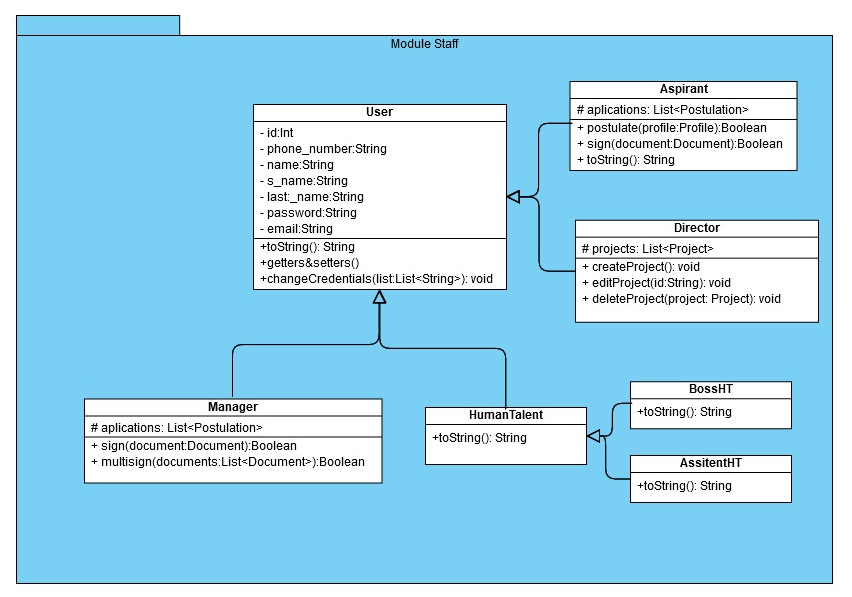
\includegraphics[width=\textwidth]{DC/DC2.jpg} 
	\caption{Package Staff, logic of users for Web Module}
	\label{fig:Clase2}
\end{figure}

\begin{figure}[H]
	\centering  \small
	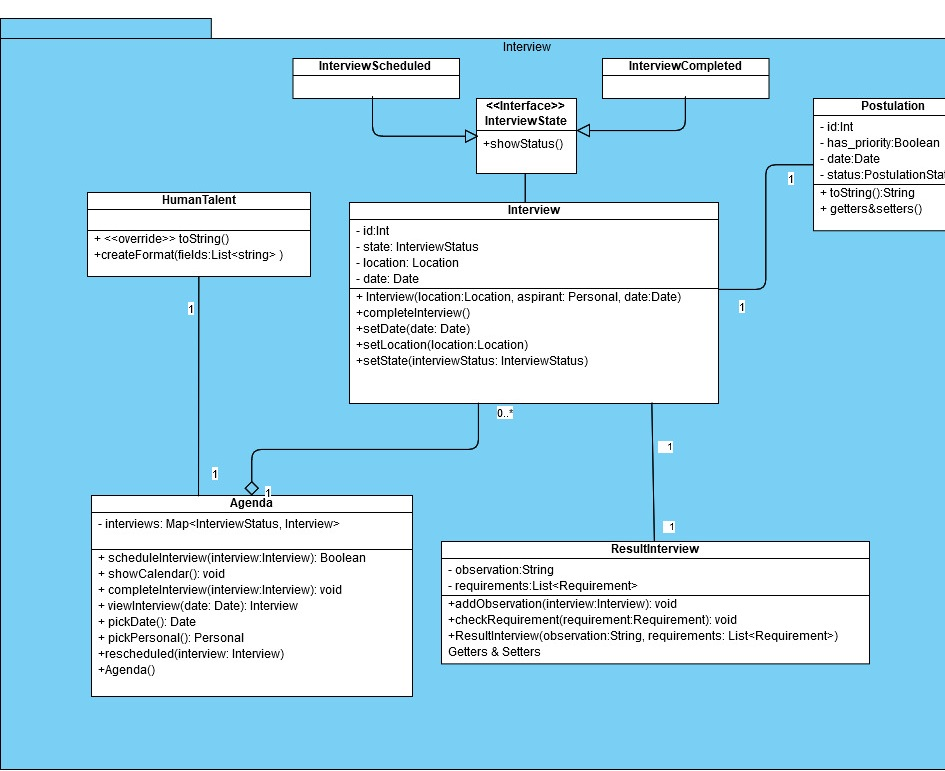
\includegraphics[width=\textwidth]{DC/DC3.jpg} 
	\caption{Package of Interview, with pattern State for the state, for Web Module}
	\label{fig:Clase3}
\end{figure}

\begin{figure}[H]
	\centering  \small
	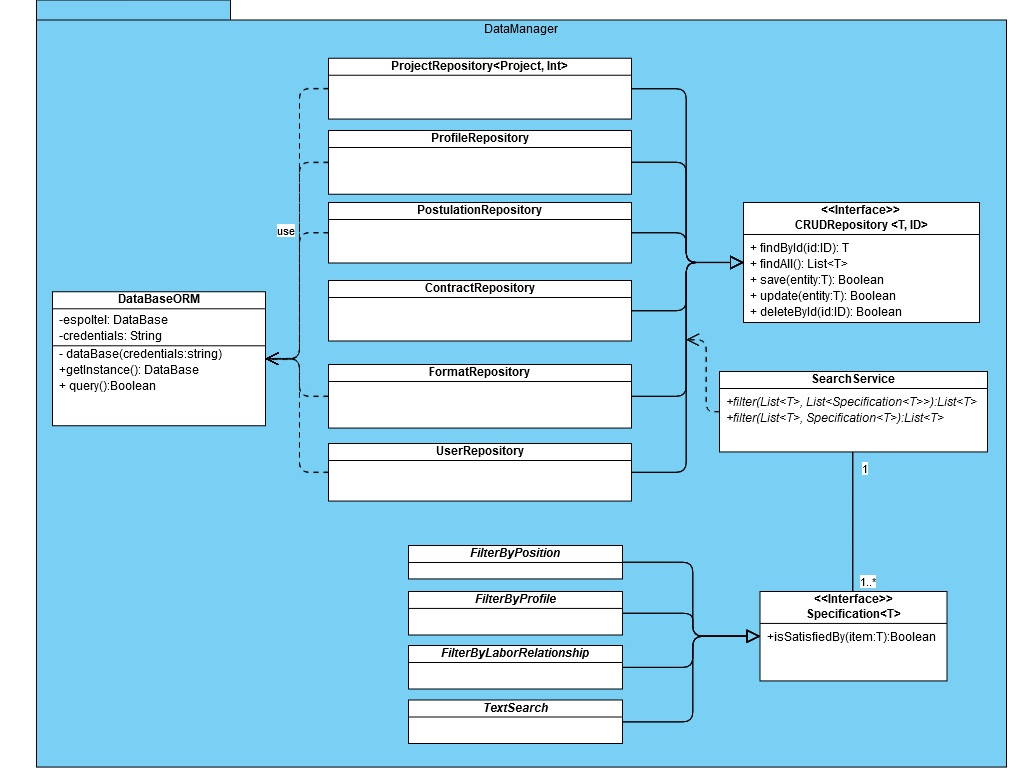
\includegraphics[width=\textwidth]{DC/DC4.jpg} 
	\caption{Package DataManager, with pattern Repository and Specification for Web Module}
	\label{fig:Clase4}
\end{figure}

\begin{figure}[H]
	\centering  \small
	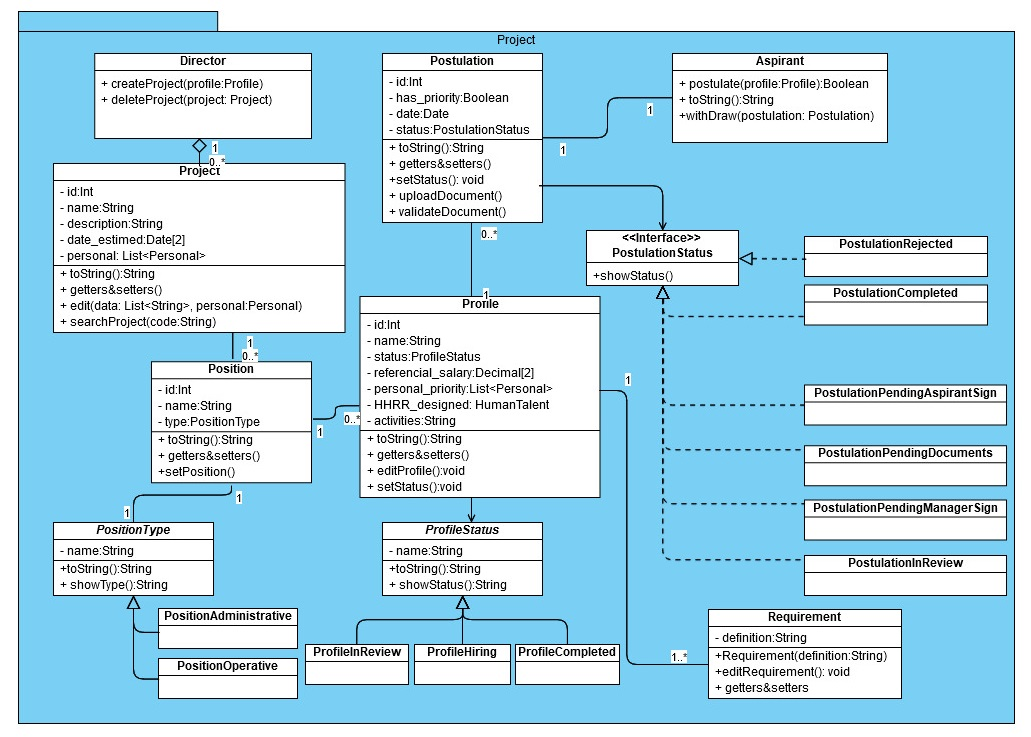
\includegraphics[width=\textwidth]{DC/DC5.jpg} 
	\caption{Package Project, with business logic of projects in ESPOLTEL for Web Module}
	\label{fig:Clase5}
\end{figure}

\begin{figure}[H]
	\centering  \small
	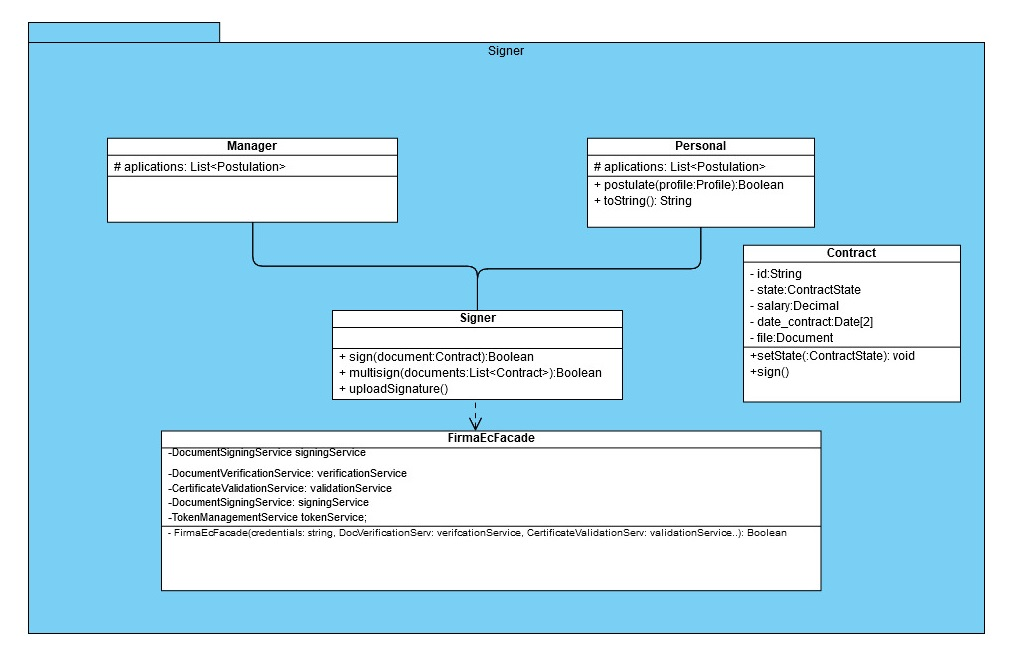
\includegraphics[width=\textwidth]{DC/DC6.jpg} 
	\caption{Package Signer, with a Facade pattern for use the FirmaEC's modules for Web Module}
	\label{fig:Clase6}
\end{figure}


\section{Class Diagram - Mobile Module}


\begin{figure}[H]
	\centering  \small
	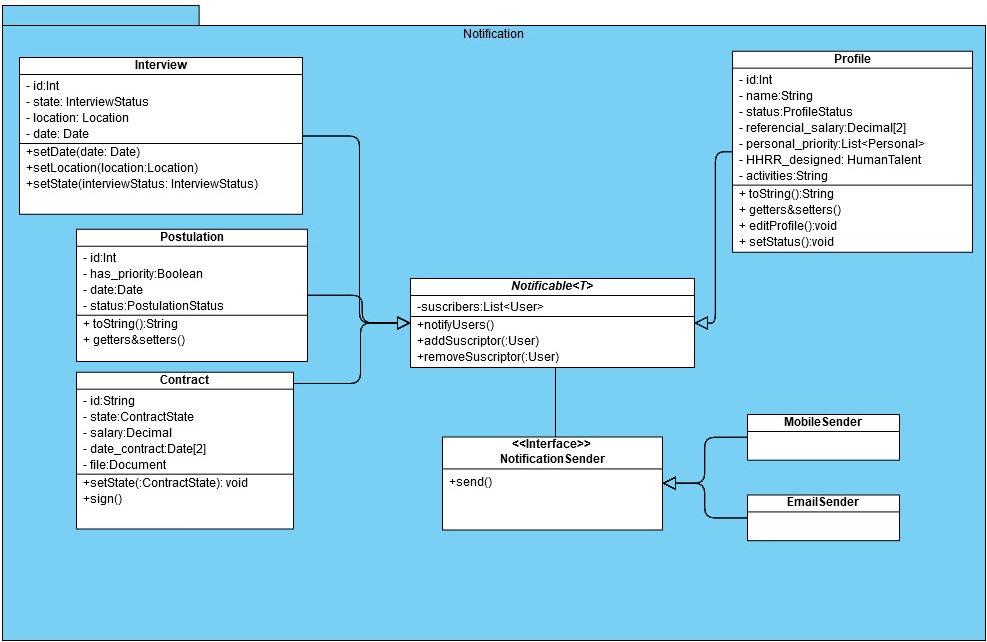
\includegraphics[width=\textwidth]{DC/DC7.jpg} 
	\caption{Package Notification, with Observer pattern for Mobile Module}
	\label{fig:Clase7}
\end{figure}

\section{Object Diagram}
 \begin{figure}[H]
	\centering  \small
	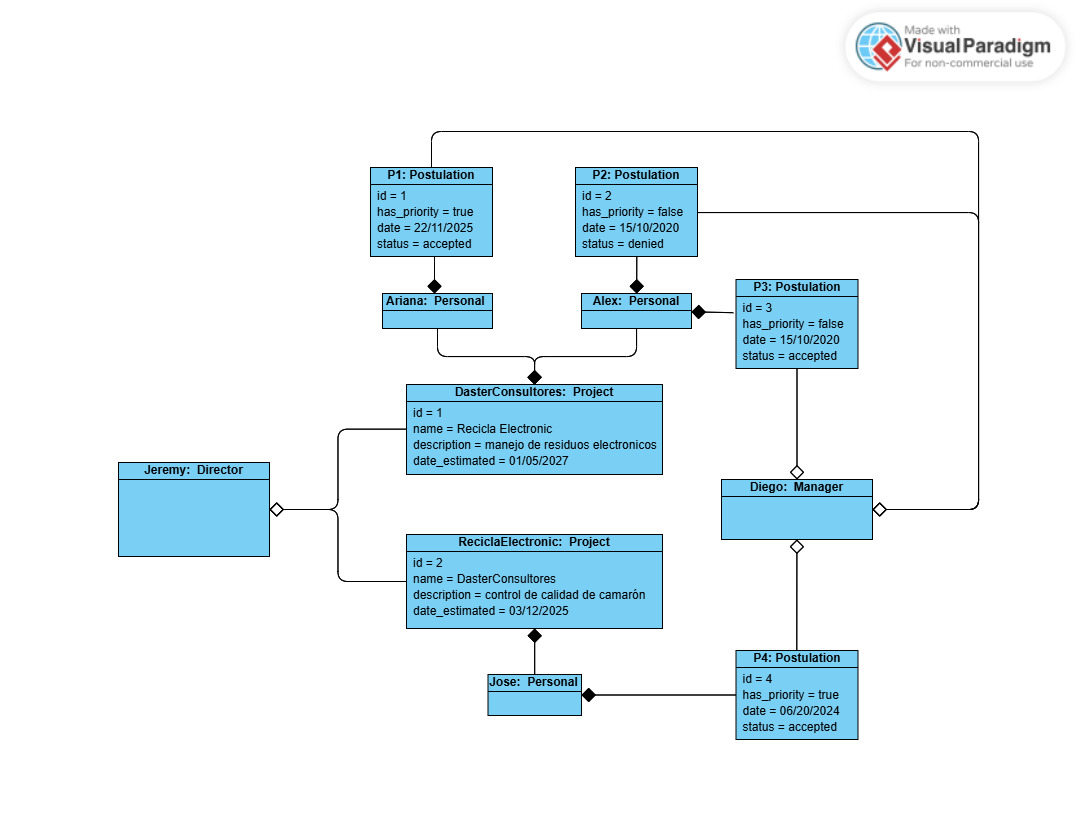
\includegraphics[width=\textwidth]{ObjectDiagram.jpeg} 
	\caption{Object Diagram of ESPOLTEL HIRING MANAGER}
	\label{fig:OBJD}
\end{figure}

\section{Component Diagram - Web Module}
 \begin{figure}[H]
	\centering  \small
	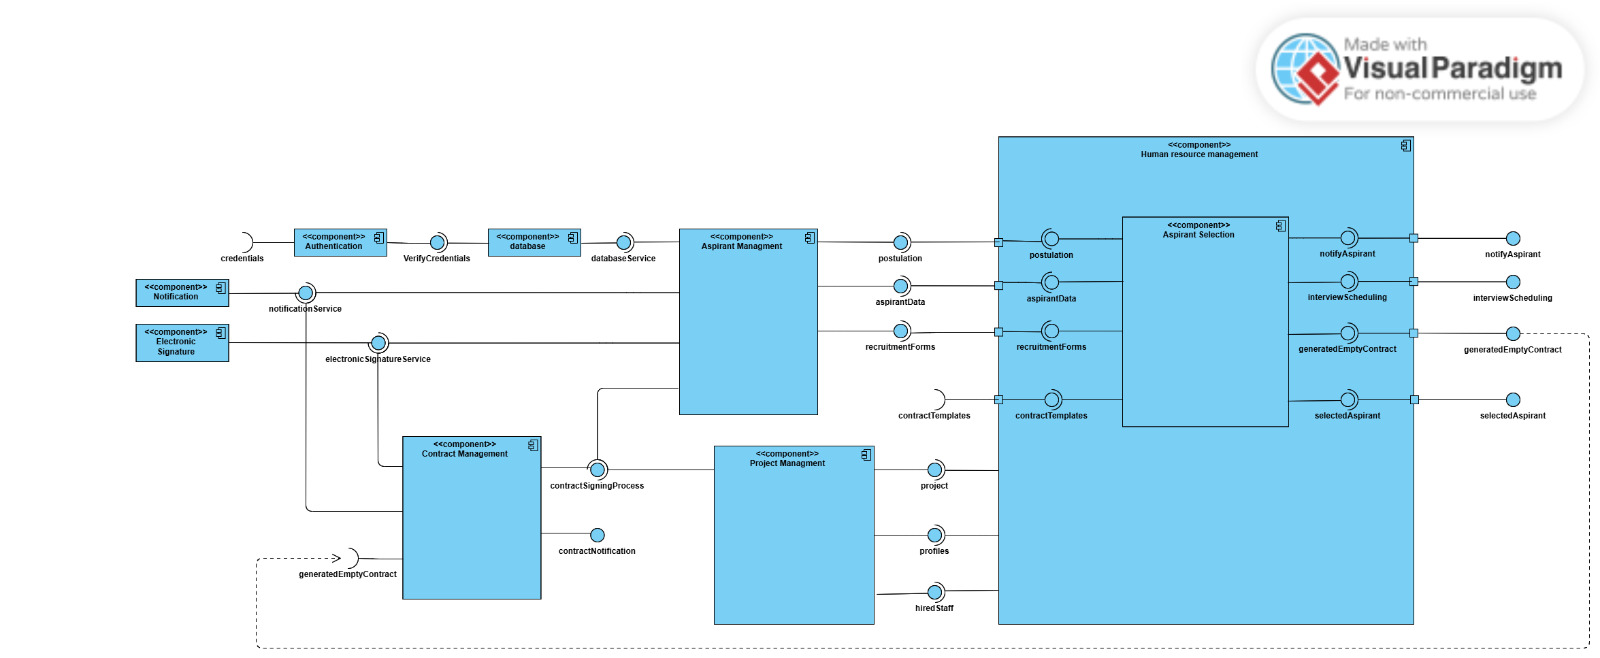
\includegraphics[width=\textwidth]{DCP/DCP1.jpeg} 
	\caption{Web module component Diagram}
	\label{fig:DCP1}
\end{figure}
\section{Component Diagram - Mobile Module}
\begin{figure}[H]
	\centering  \small
	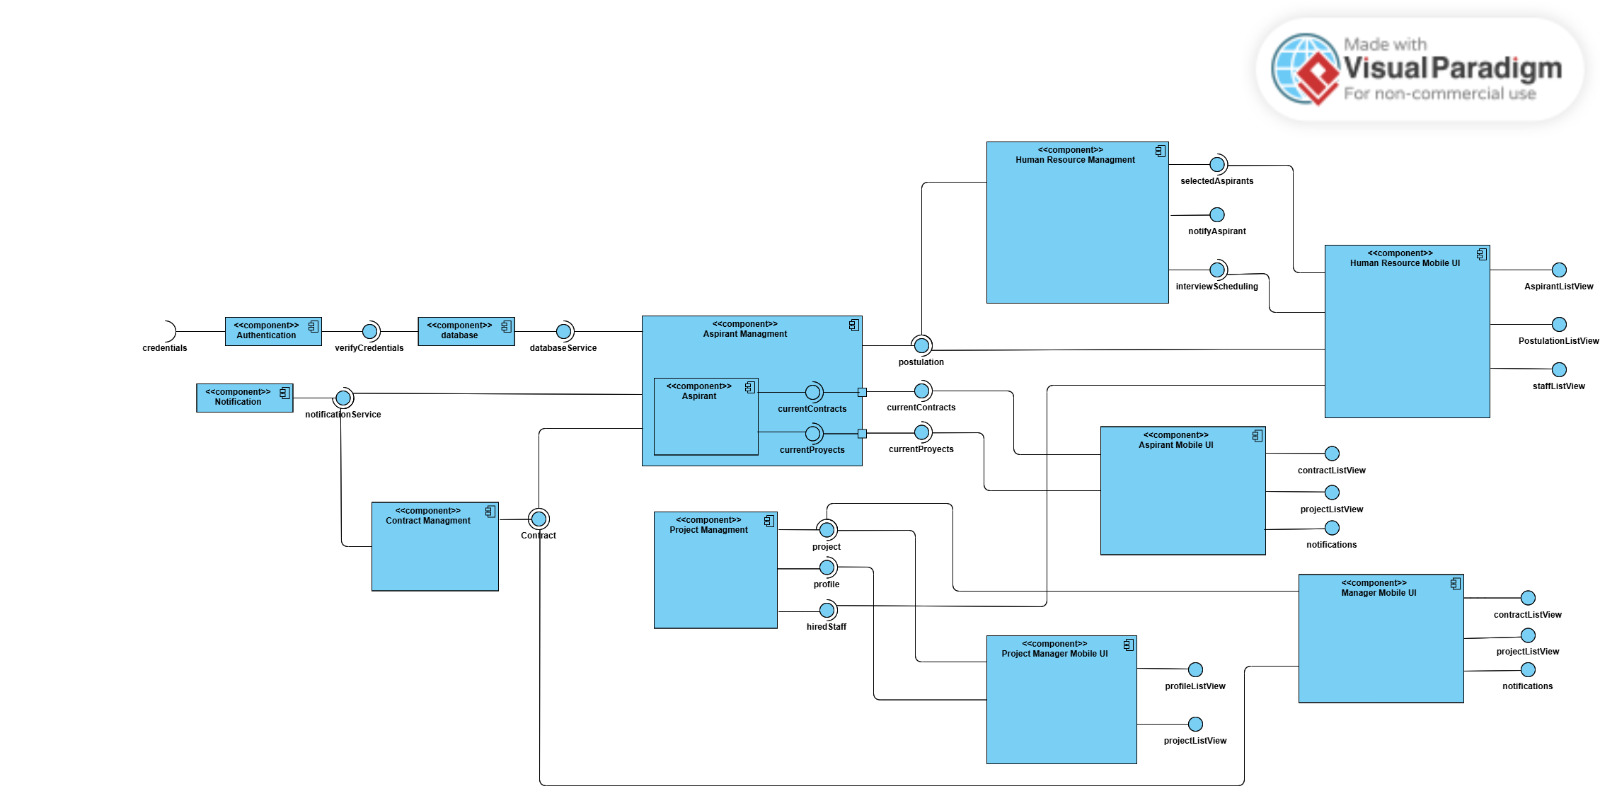
\includegraphics[width=\textwidth]{DCP/DCP2.jpeg} 
	\caption{Mobile module component Diagram}
	\label{fig:DCP2}
\end{figure}

\section{Deployment Diagram - Web Module}
\begin{figure}[H]
	\centering  \small
	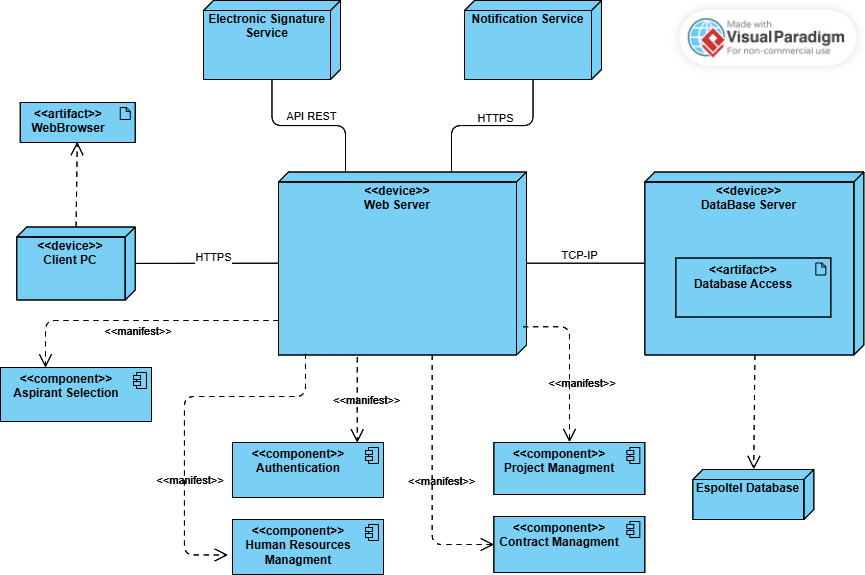
\includegraphics[width=\textwidth]{DPL/DPL1.jpeg} 
	\caption{Web module deployment Diagram}
	\label{fig:DPL1}
\end{figure}
\section{Deployment Diagram - Mobile Module}
\begin{figure}[H]
	\centering  \small
	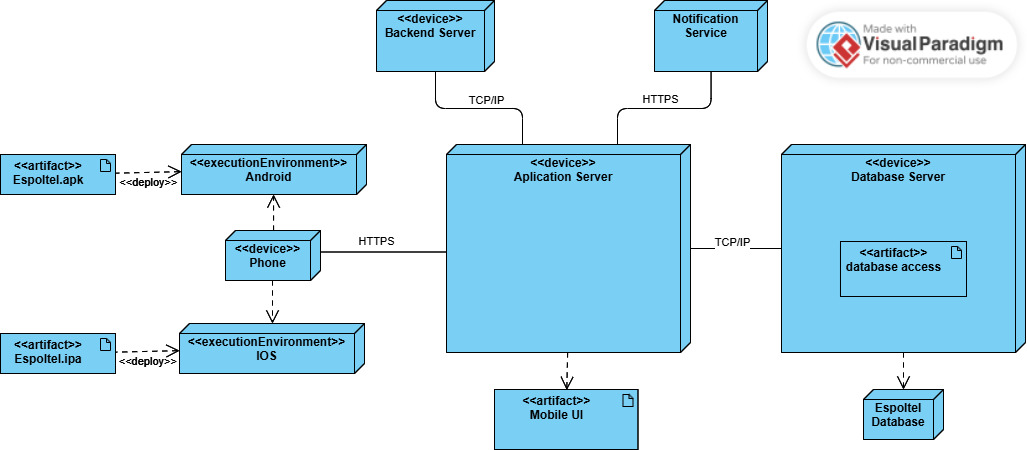
\includegraphics[width=\textwidth]{DPL/DPL2.jpeg} 
	\caption{Mobile module deployment Diagram}
	\label{fig:DPL2}
\end{figure}
\chapter{Behavior UML}

\section{Activity Diagram}
\begin{figure}[H]
	\centering
	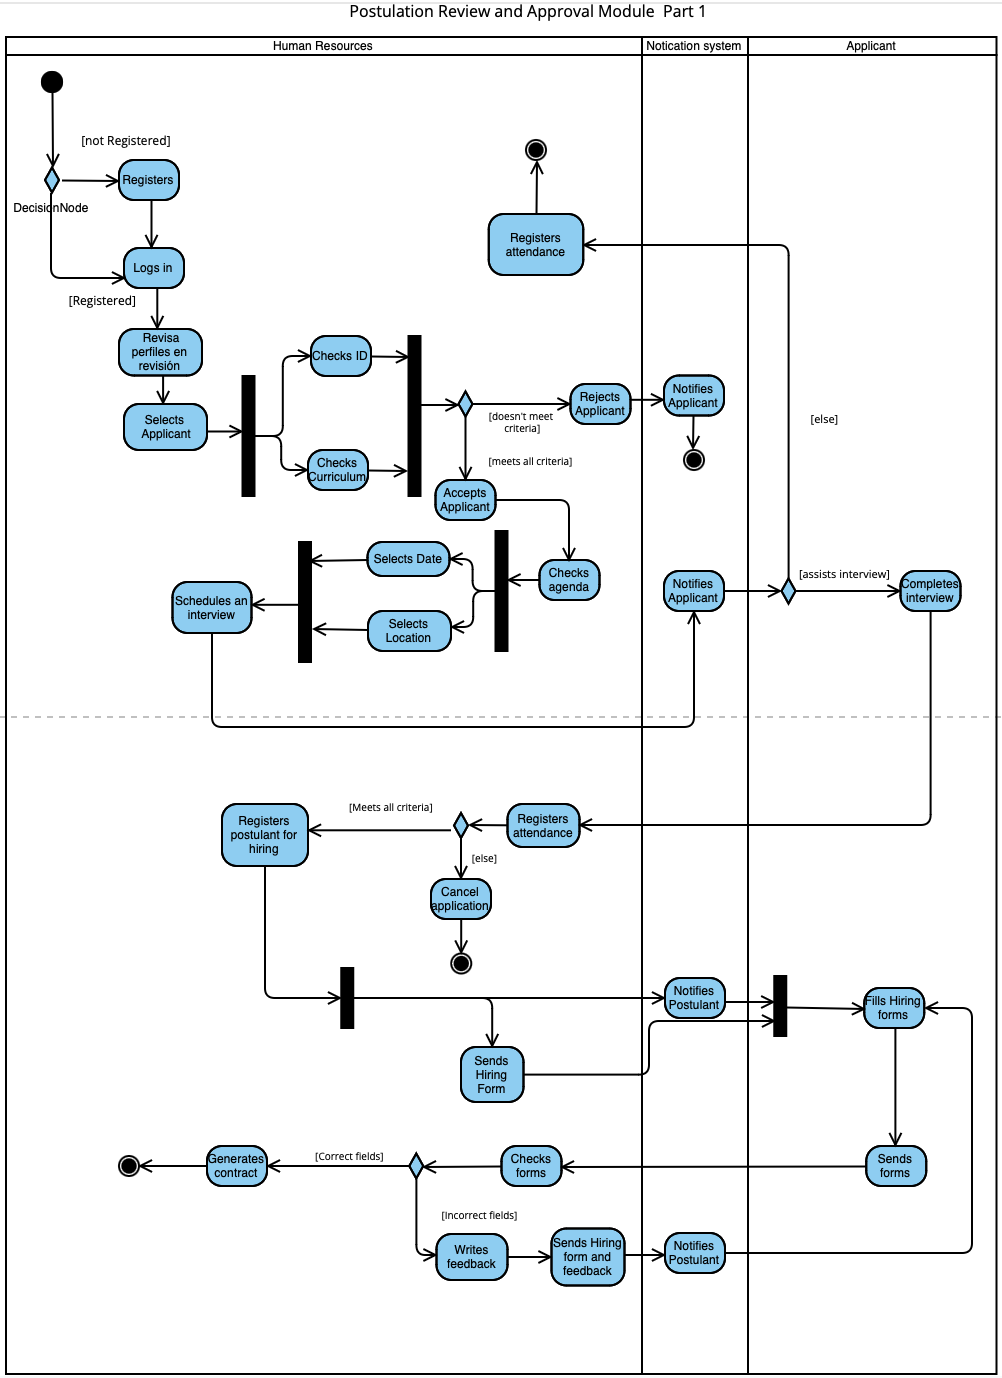
\includegraphics[width=\textwidth]{AD/AD1.png}
	\caption{Activity Diagram: Postulation review, Part one}
	\label{fig:AD1}
\end{figure}

\begin{figure}[H]
	\centering
	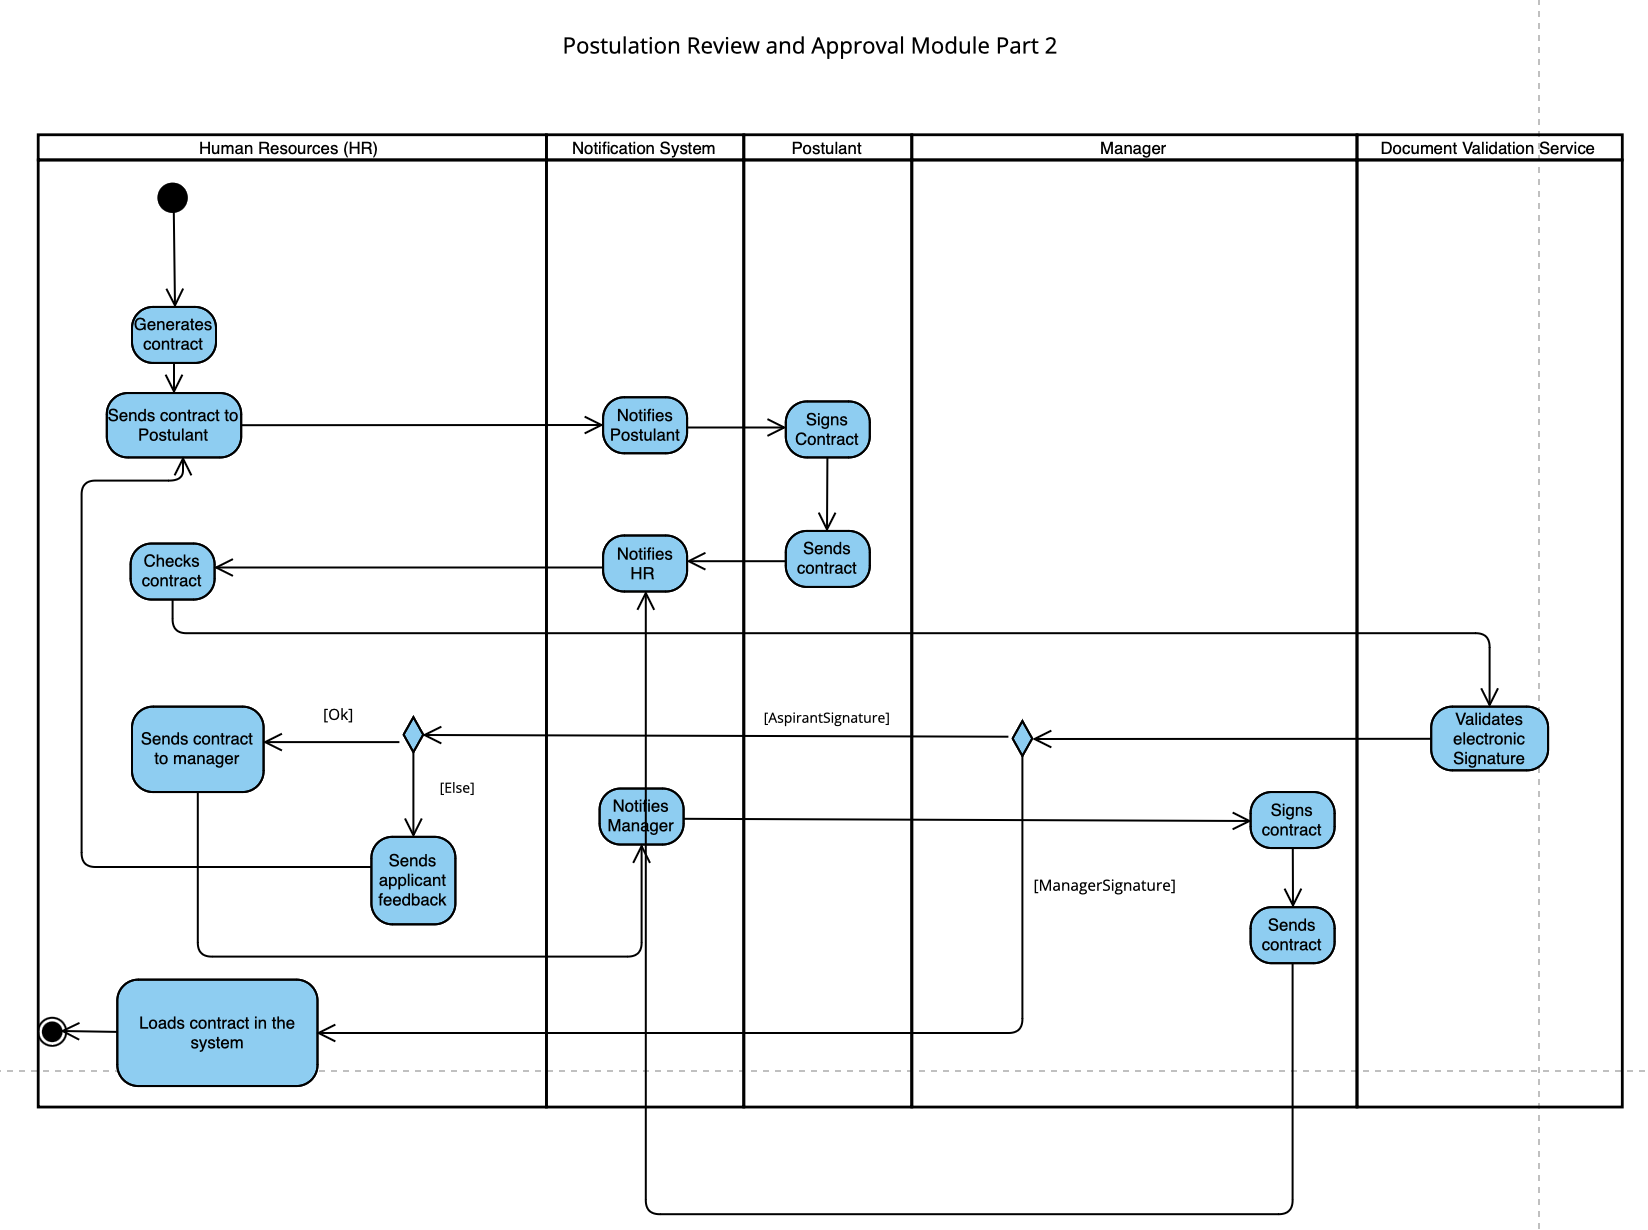
\includegraphics[width=\textwidth]{AD/AD2.png}
	\caption{Activity Diagram: Postulation review, Part two}
	\label{fig:AD2}
\end{figure}

\begin{figure}[H]
	\centering
	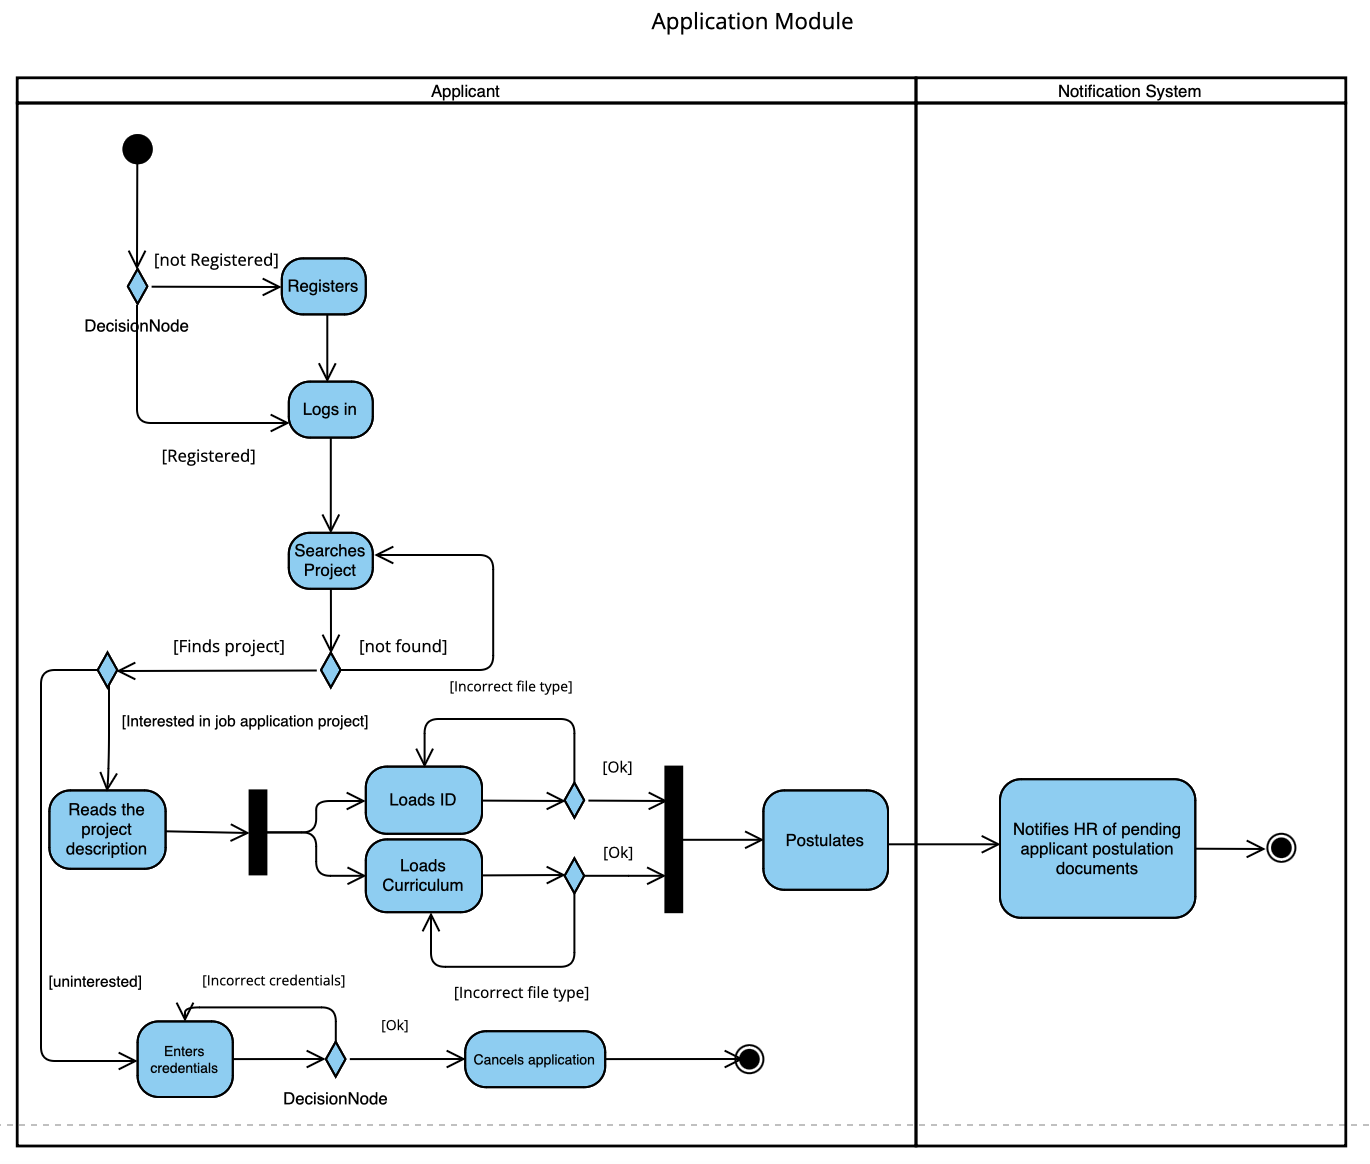
\includegraphics[width=\textwidth]{AD/AD3.png}
	\caption{Activity Diagram: Make an Application/Postulation}
	\label{fig:AD3}
\end{figure}

\begin{figure}[H]
	\centering
	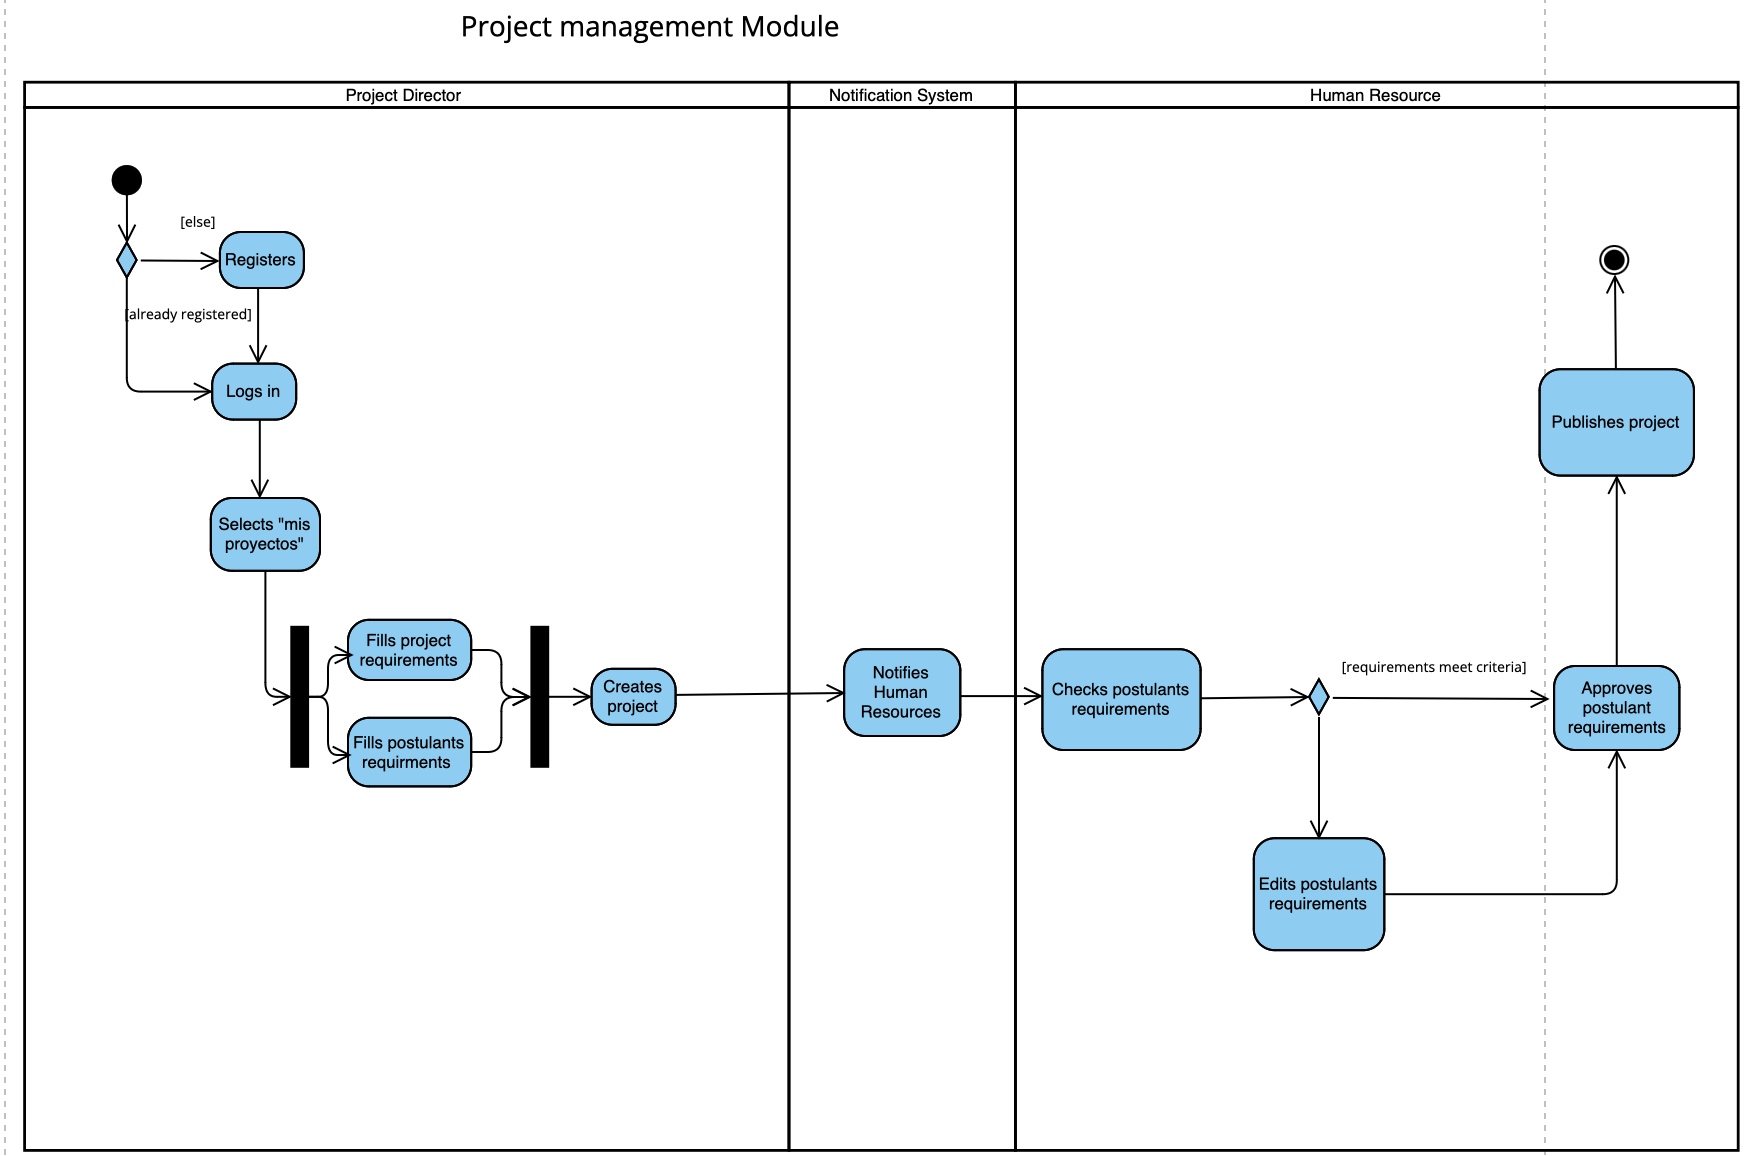
\includegraphics[width=\textwidth]{AD/AD4.png}
	\caption{Activity Diagram: Management of a project}
	\label{fig:AD4}
\end{figure}

\section{Sequence Diagram}

\foreach \i in {0,...,32} {
	\begin{figure}[H]
		\centering
		\includegraphics[width=\textwidth]{SD/SD\i.png}
		\caption{Sequence Diagram \i}
		\label{fig:SD\i}
	\end{figure}
}

\section{Status Diagram}
\begin{figure}[H]
	\centering
	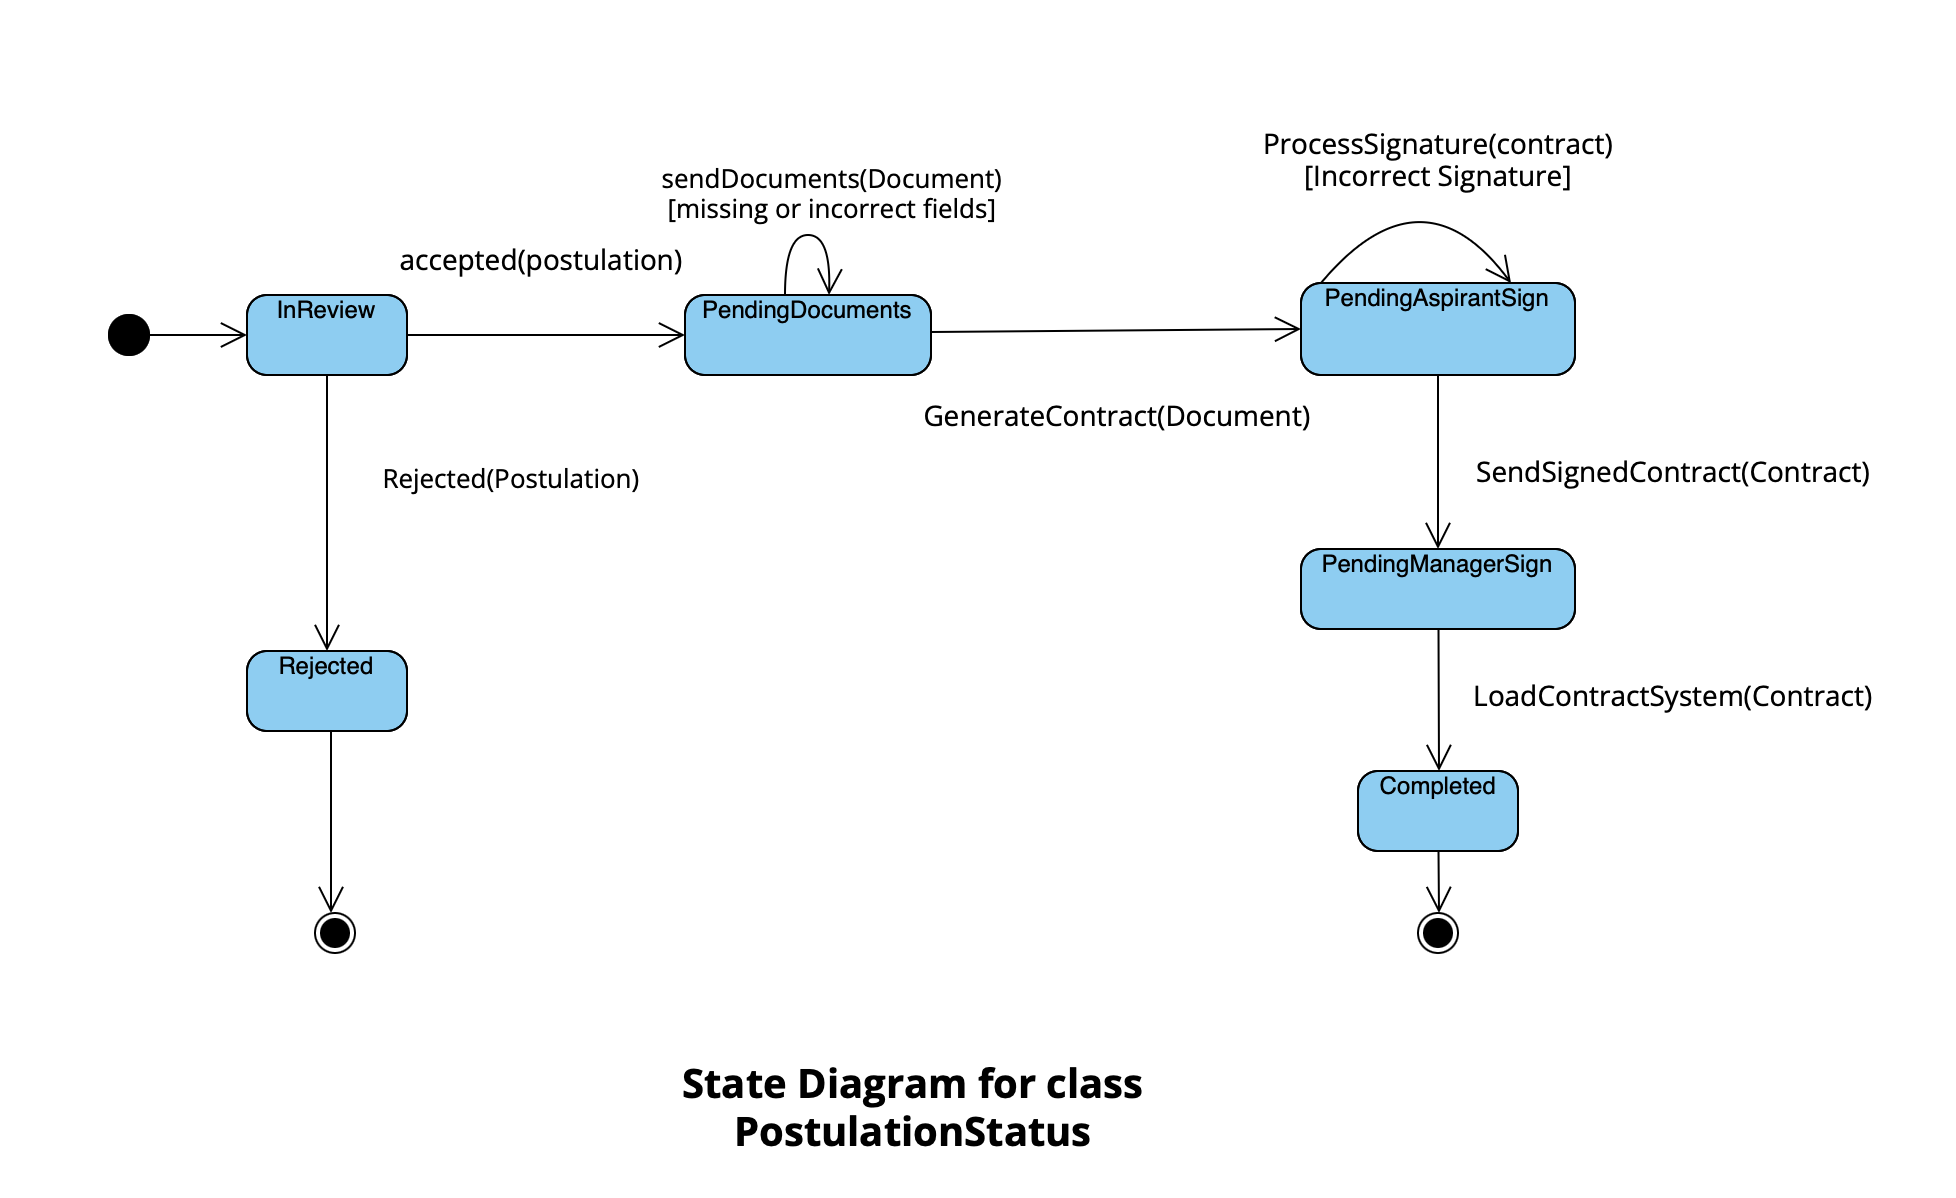
\includegraphics[width=\textwidth]{ST/ST1.png}
	\caption{State Diagram: for Postulation status}
	\label{fig:ST1}
\end{figure}

\begin{figure}[H]
	\centering
	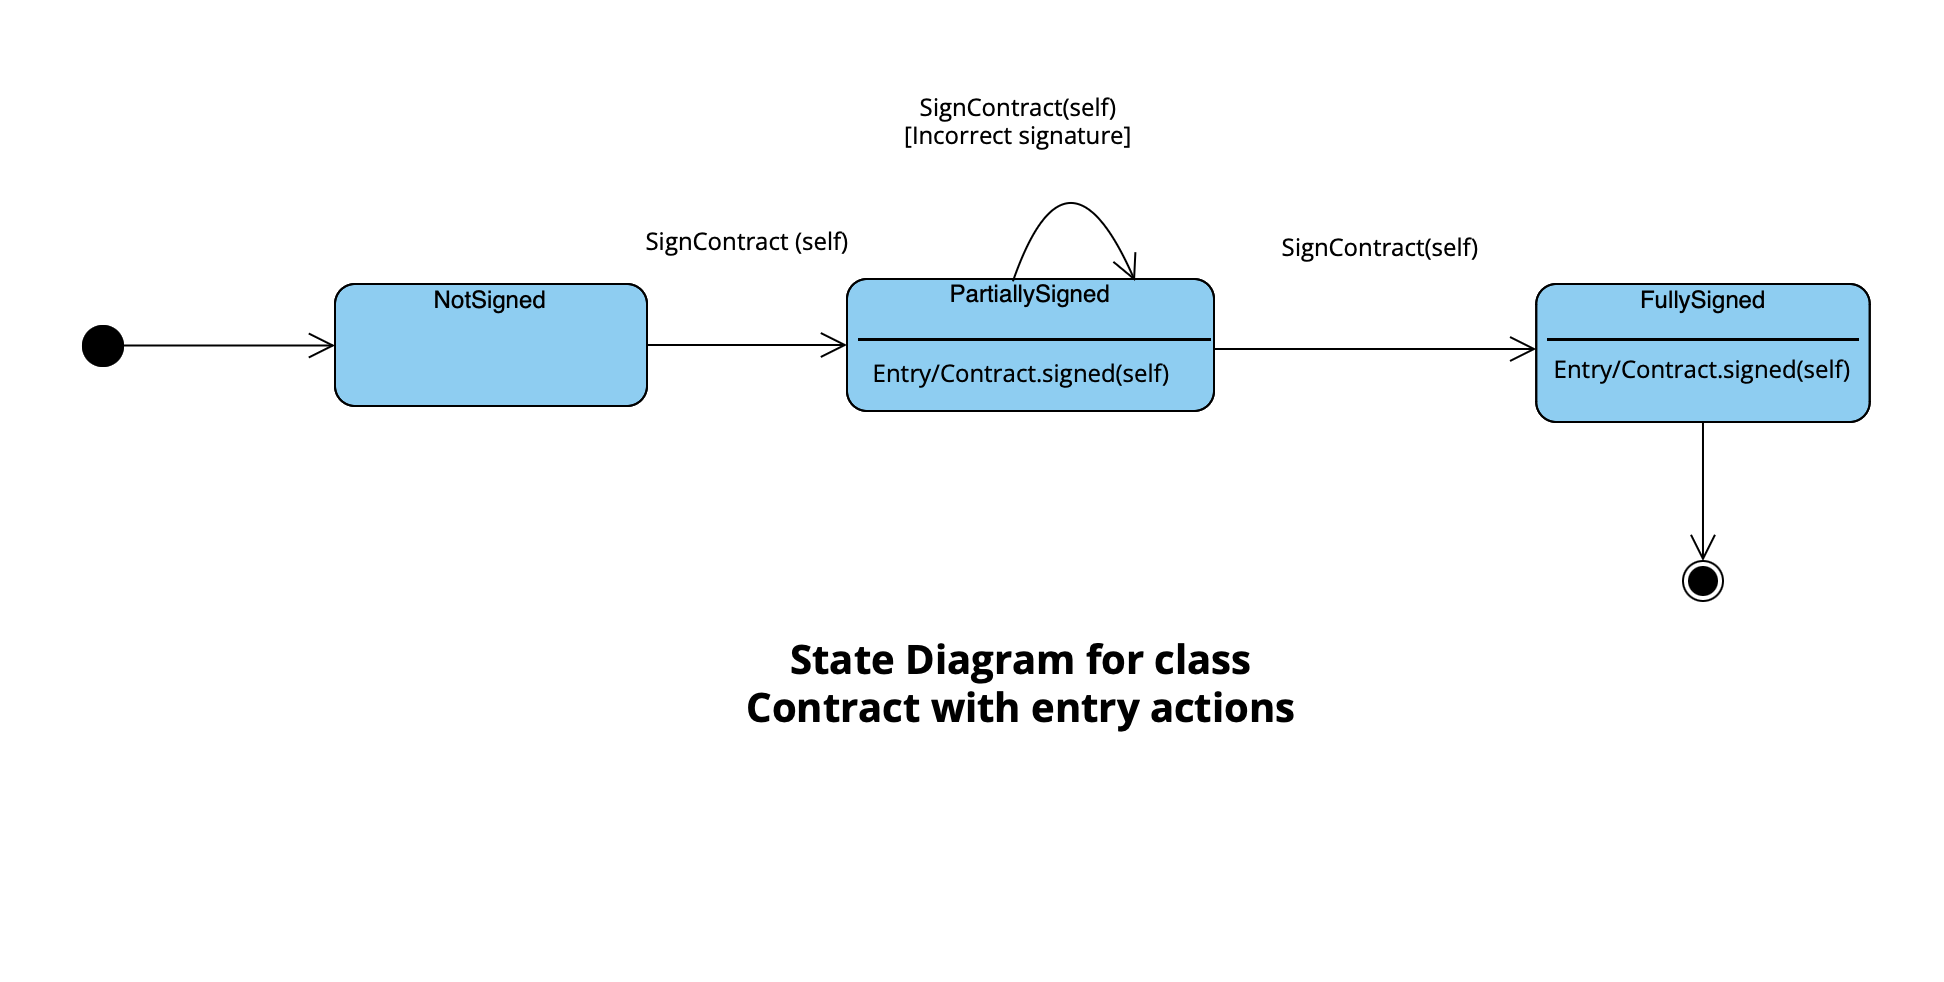
\includegraphics[width=\textwidth]{ST/ST2.png}
	\caption{State Diagram: for Contract status}
	\label{fig:ST2}
\end{figure}

\begin{figure}[H]
	\centering
	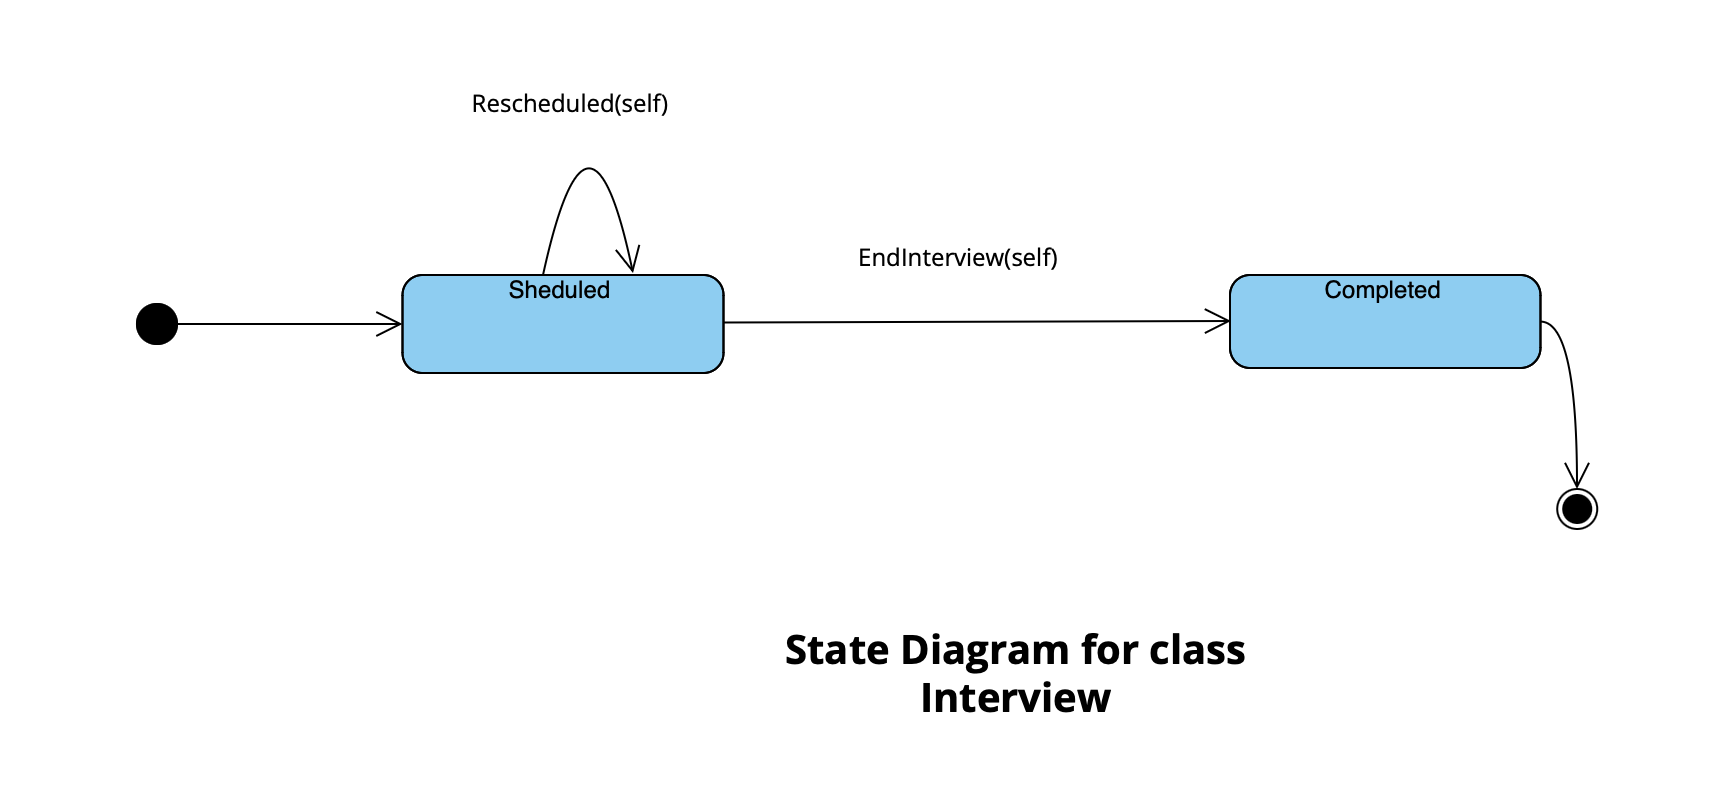
\includegraphics[width=\textwidth]{ST/ST3.png}
	\caption{State Diagram: for Interview status}
	\label{fig:ST3}
\end{figure}

\section{Collaboration Diagram}


\chapter{Individual Contributions}
\vspace{2cm}

\begin{table}[h!]
    \centering \small
    \renewcommand{\arraystretch}{1.5} 
    \begin{tabular}{|p{5cm}|p{10cm}|} 
    \hline
    \textbf{Student's Names} & \textbf{Contributions} \\ \hline
    Jeremy Rodrigo Poveda Gorotiza & Risk Management, Product, Sprint backlog, review and creation of LaTeX document, class diagrams with patterns, use case documentation. \\ \hline
    Diego Fernando Flores Rengifo & Creation of use cases, activity diagrams, state diagrams, class diagrams, sequence diagrams, and collaboration diagram help. \\ \hline
    José David Ramos Rios & Creation of sequence diagrams, creation of "interview" module in class diagram, product backlog review, documentation of use case diagrams. \\ \hline
    Ariana Valentina Palacios Saenz & Review document, creation of object, component, deployment and collaboration diagrams\\ \hline
    Alex Javier Vizuete Pereira & Creation of use cases, sequence diagrams, document revision, help with recompiling images, help with the collaboration diagram.\\ \hline
    \end{tabular}
    \caption{Responsibilities of each member of team 3}
\end{table} \FloatBarrier 



\chapter{Appendix}

\section{Appendix A: Github Repository}
The versioning of the project prototype has been managed using Github. You can find it through the following link ESPOLTEL's versioning project:\\ \href{https://github.com/Jeremy-Poveda/EspoltelHiringManager}{Repository link}
\section{Appendix B: Acceptance Documents Agreement}
 \begin{figure}[H]
 	\centering  \small
 	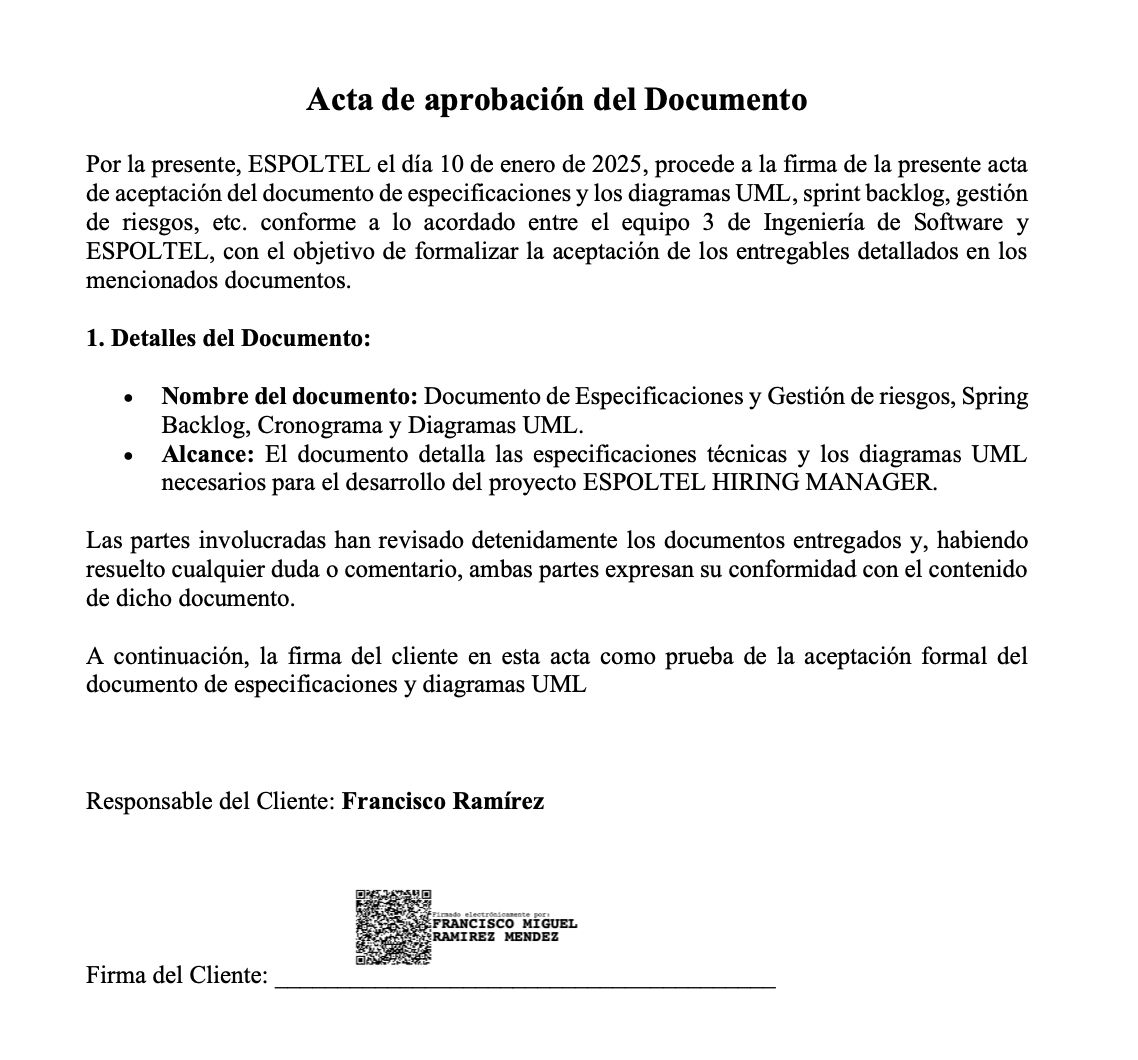
\includegraphics[width=\textwidth]{Acceptance.jpeg} 
 	\caption{Acceptance of the client, Francisco Ramirez}
 	\label{fig:Acceptance}
 \end{figure}
\FloatBarrier 
\section{Appendix C: Tools used}
\begin{table}[H]
	\centering
	\begin{tabular}{|p{5cm}|p{5cm}|}
		\hline
		\textbf{Tool} & \textbf{Description} \\ \hline
		Visual Paradigm & A comprehensive tool used for creating various UML diagrams, ER diagrams, and flowcharts. It supports both software modeling and system design. \\ \hline
		pLaTeX & A tool for high-quality typesetting in LaTeX, often used for documents, academic papers, and presentations with a focus on clear formatting and mathematical typesetting. \\ \hline
		SequenceDiagram.org & An online tool for creating and visualizing sequence diagrams, often used to model interactions between different parts of a system in a step-by-step manner. \\ \hline
	\end{tabular}
	\caption{Diagramming Tools Used}
	\label{table:DiagrammingTools}
\end{table}



\end{document}

